%!TEX root = ../thesis.tex
% ******************************* Thesis Appendix A ****************************
\chapter{Schematics of the iPG instrument} 


\ifpdf
\graphicspath{{Appendix1/Figs/Raster/}{Appendix1/Figs/PDF/}{Appendix1/Figs/}}
\else
\graphicspath{{Appendix1/Figs/Vector/}{Appendix1/Figs/}}
\fi

\section*{Power supply}
\label{Appendix: Power Supply}
\begin{figure}[!htpb]
	\centering
	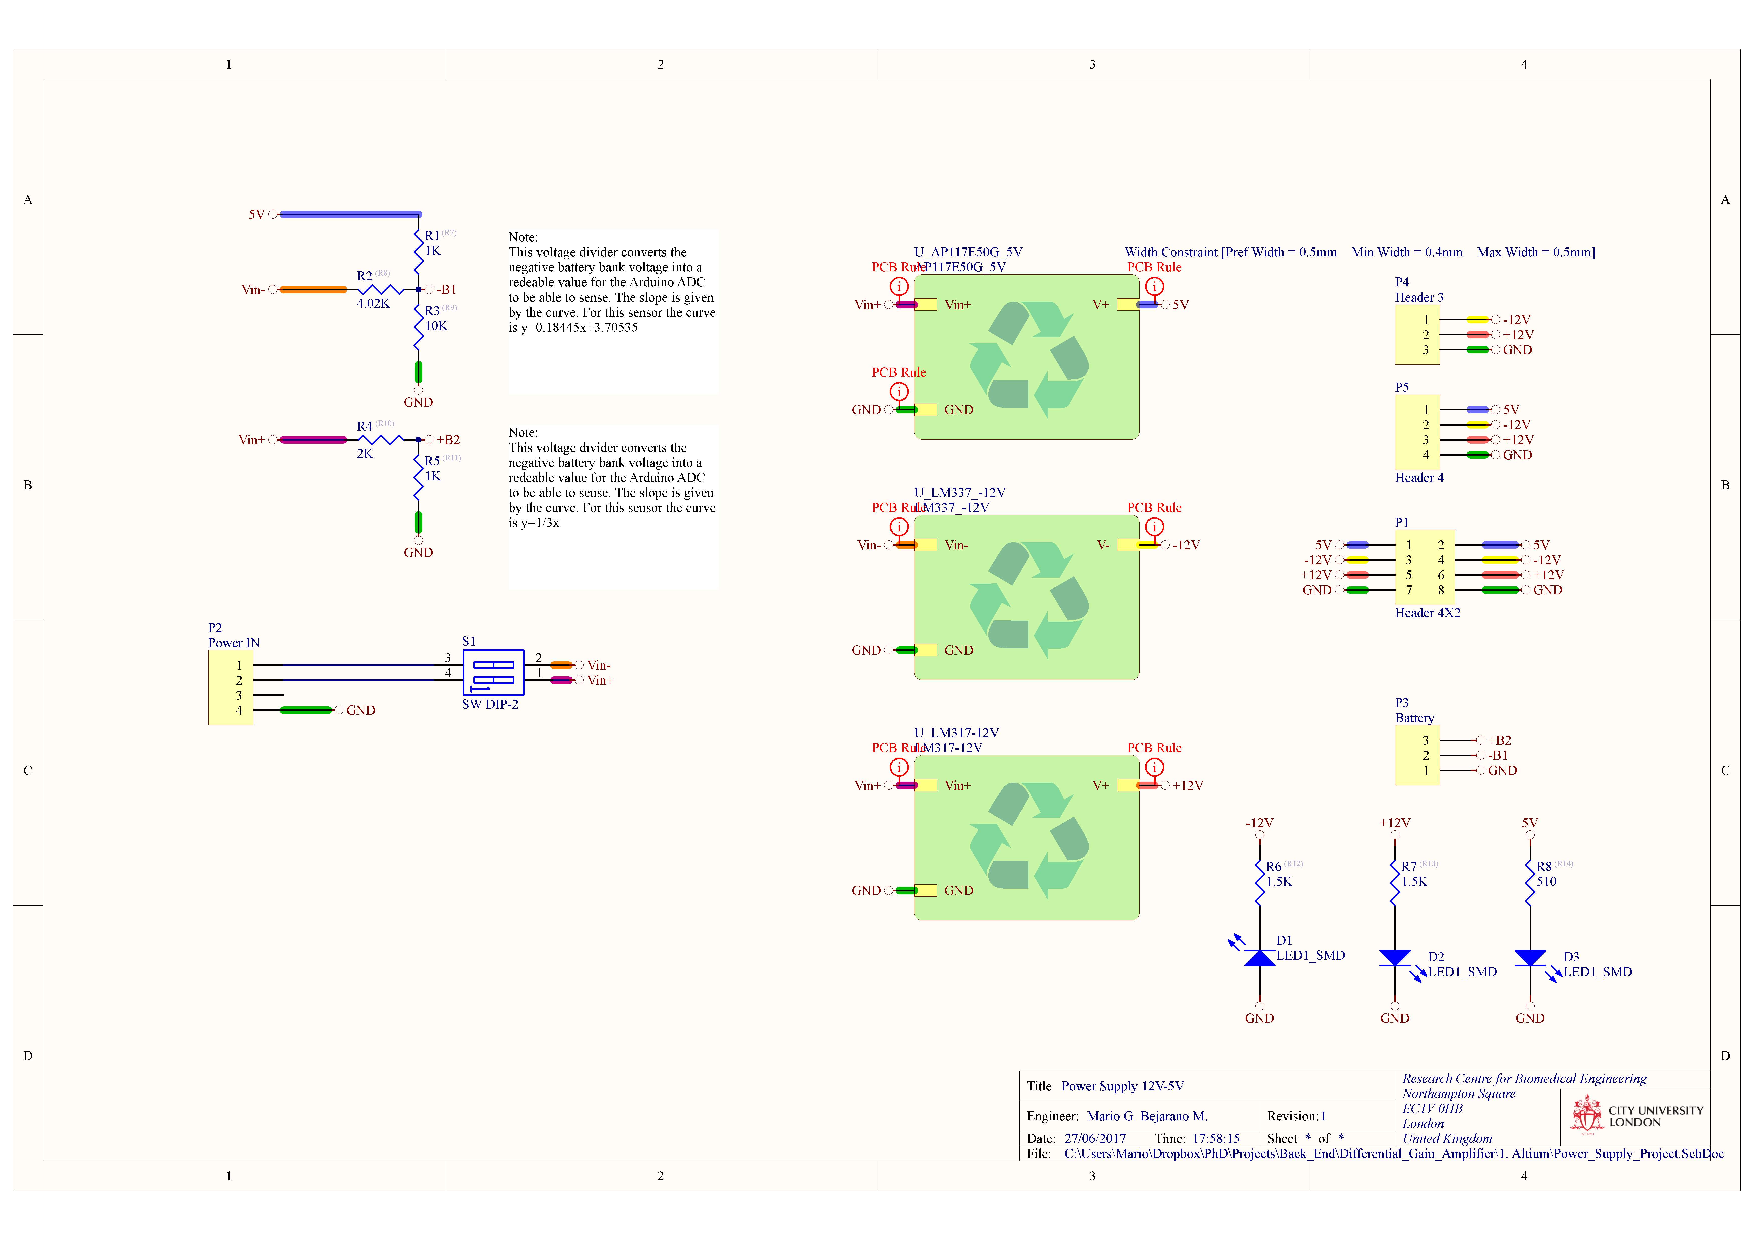
\includegraphics[width=0.55\paperwidth,keepaspectratio, angle=90]{power_supply_top}
	\caption[Top-up view of the power supply]{Top-up view of the power supply. Each box represents the Voltage regulators circuits. The schematic also includes indicators LED, switches and output ports.}
	\label{fig:schematic PS}
\end{figure}

\begin{landscape}
\begin{figure}[!htpb]
	\centering
	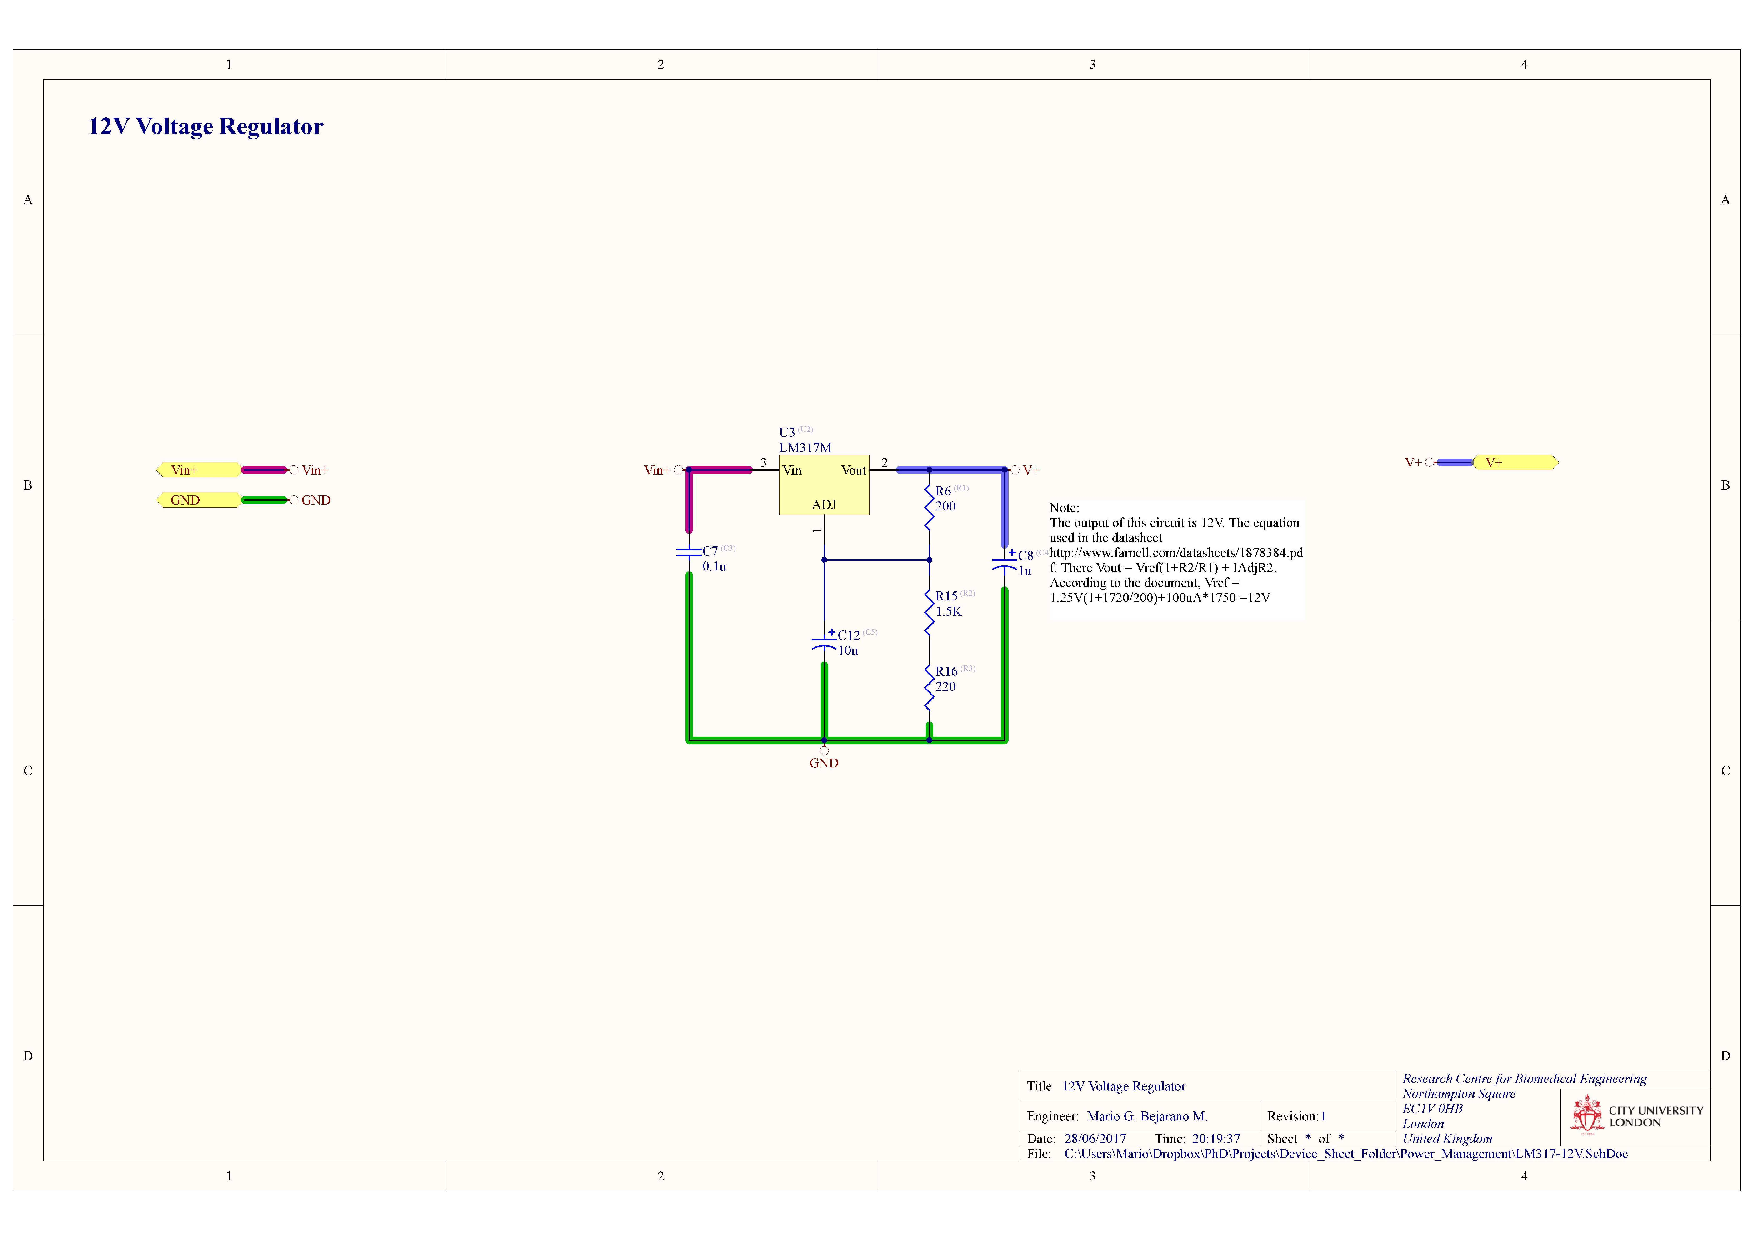
\includegraphics[width=0.95\paperwidth,keepaspectratio]{power_supply_12}
	\caption[Schematic of the \SI{12}{\volt} voltage regulator]{The schematic shows the configuration of the voltage regulator LM317, the resistors selected set the output voltage at \SI{12}{\volt}. The capacitors filter ripples from the batteries.}
	\label{fig:schematic PS 12}
\end{figure}
\end{landscape}

\begin{landscape}
\begin{figure}[!htpb]
	\centering
	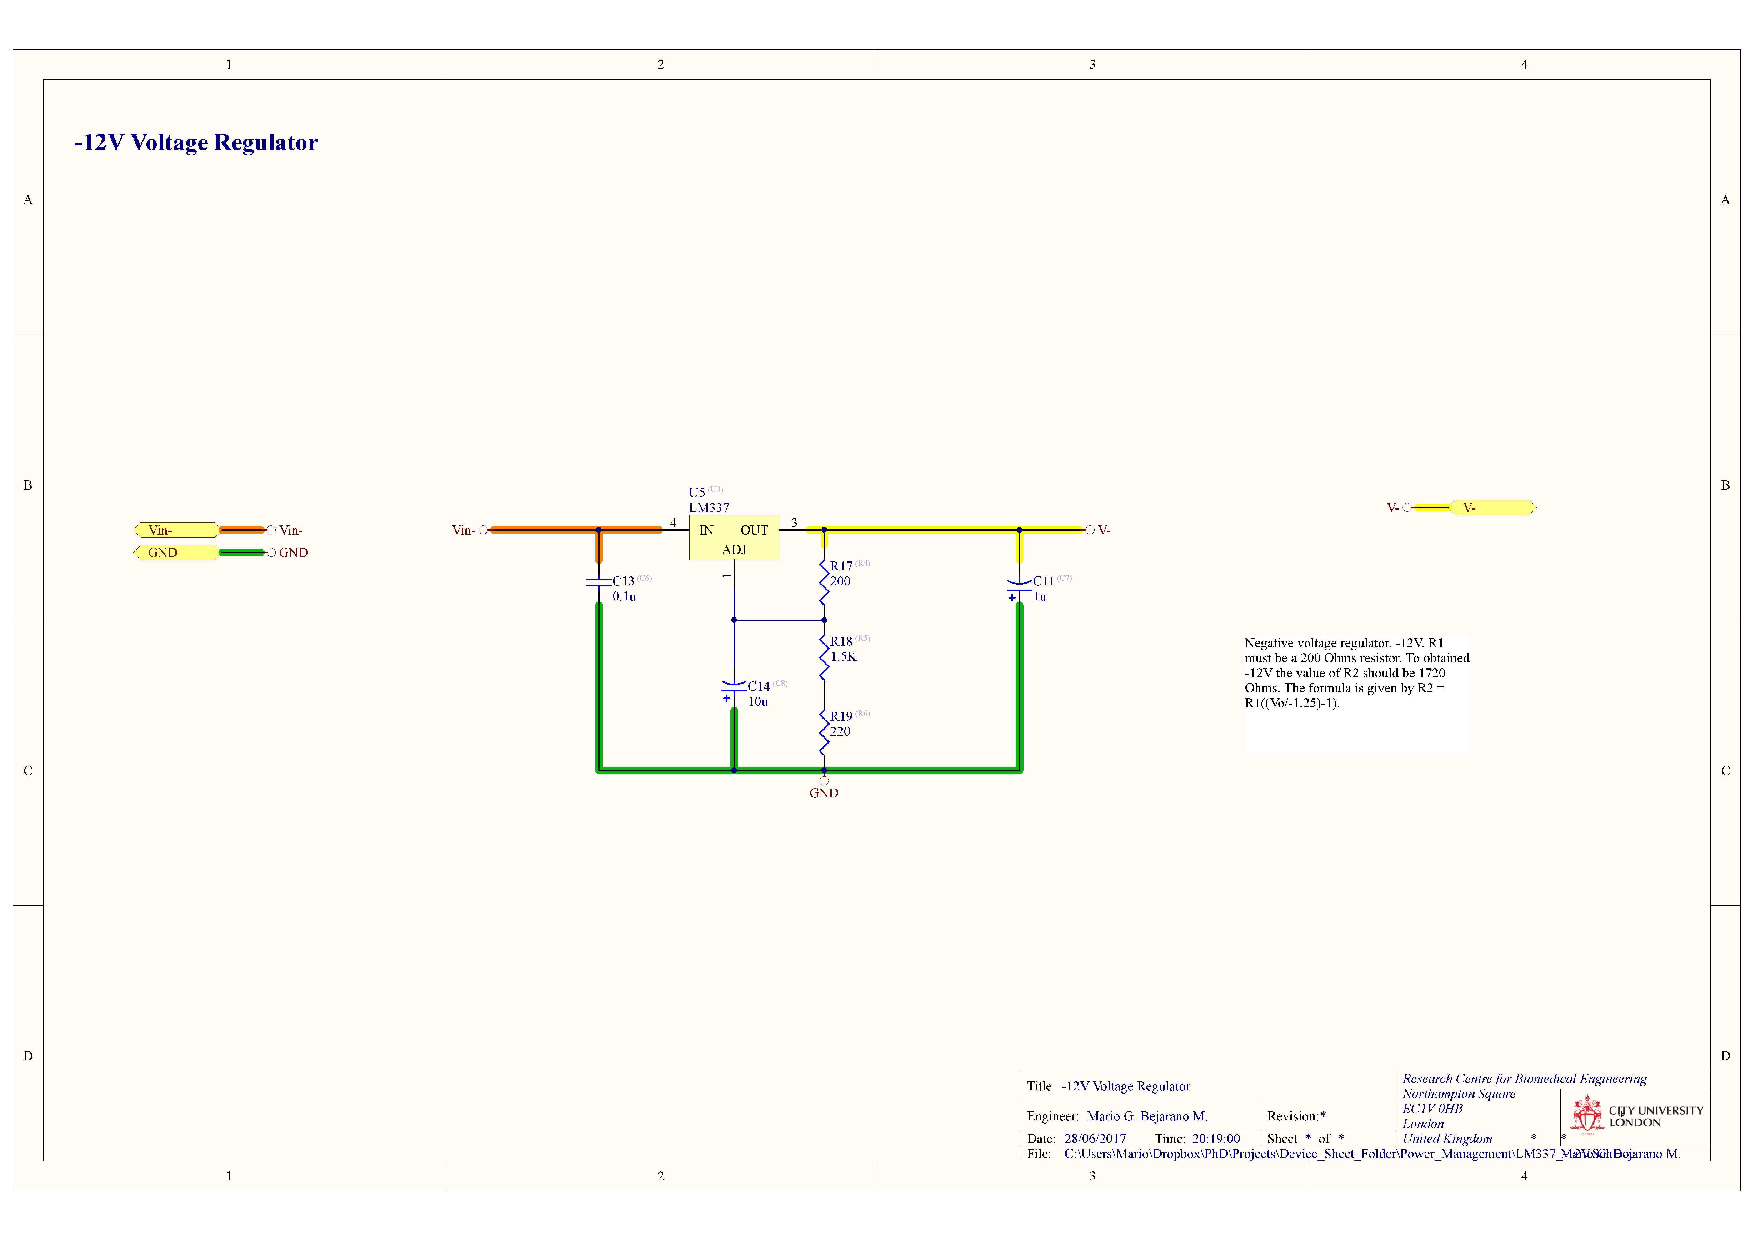
\includegraphics[width=0.95\paperwidth,keepaspectratio]{power_supply_N12}
	\caption[Schematic of the -\SI{12}{\volt} voltage regulator]{The schematic shows the configuration of the voltage regulator LM337, the resistors selected set the output voltage at -\SI{12}{\volt}. The capacitors filter noise peaks.}
	\label{fig:schematic PS N12}
\end{figure}
\end{landscape}

\begin{landscape}
\begin{figure}[!htpb]
	\centering
	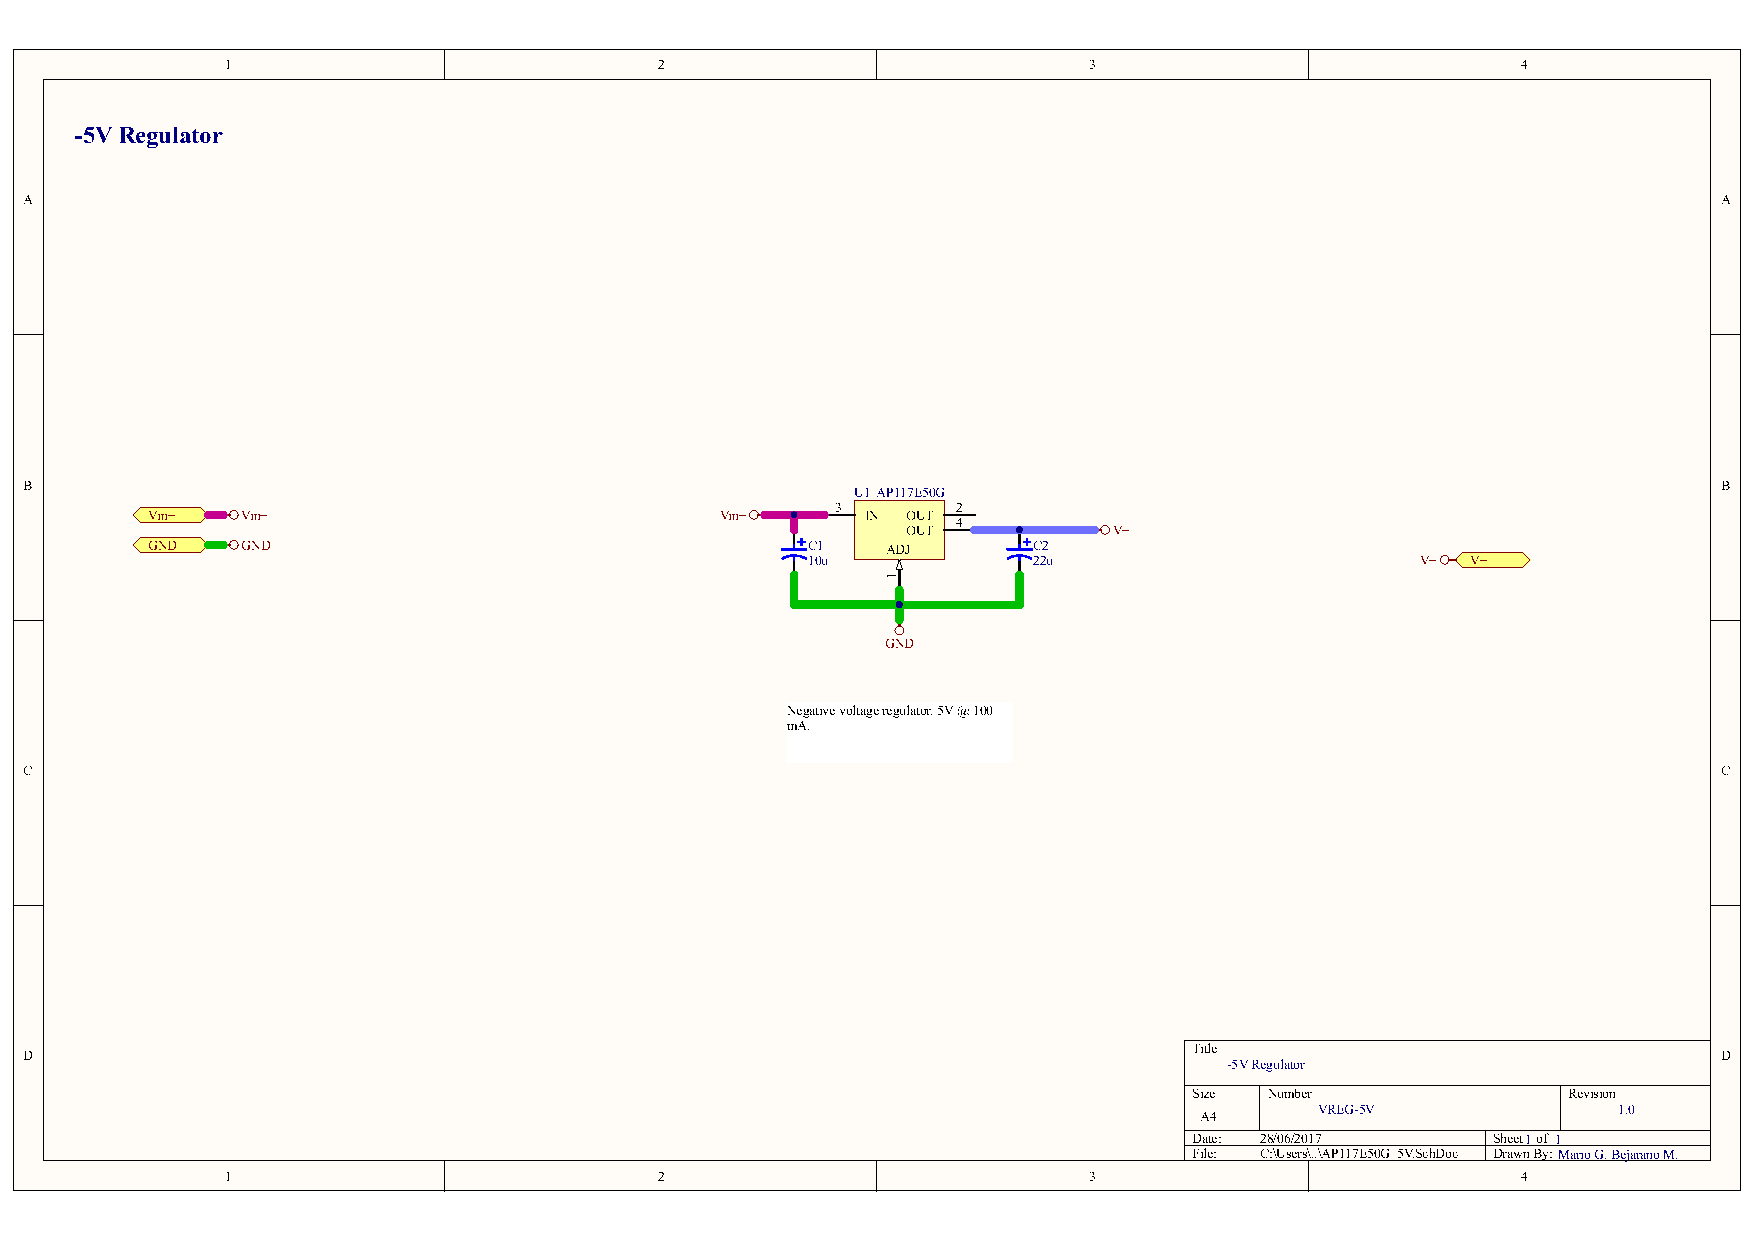
\includegraphics[width=0.95\paperwidth,keepaspectratio]{power_supply_5}
	\caption[Schematic of the \SI{5}{\volt} voltage regulator]{The schematic shows the configuration of the voltage regulator AL117E50G, the output is fixed to \SI{5}{\volt}. The capacitors filter noises from the power bank.}
	\label{fig:schematic PS 5}
\end{figure}
\end{landscape}


\section*{DDS}
\label{Appendix: DDS PS}
\begin{figure}[!htpb]
	\centering
	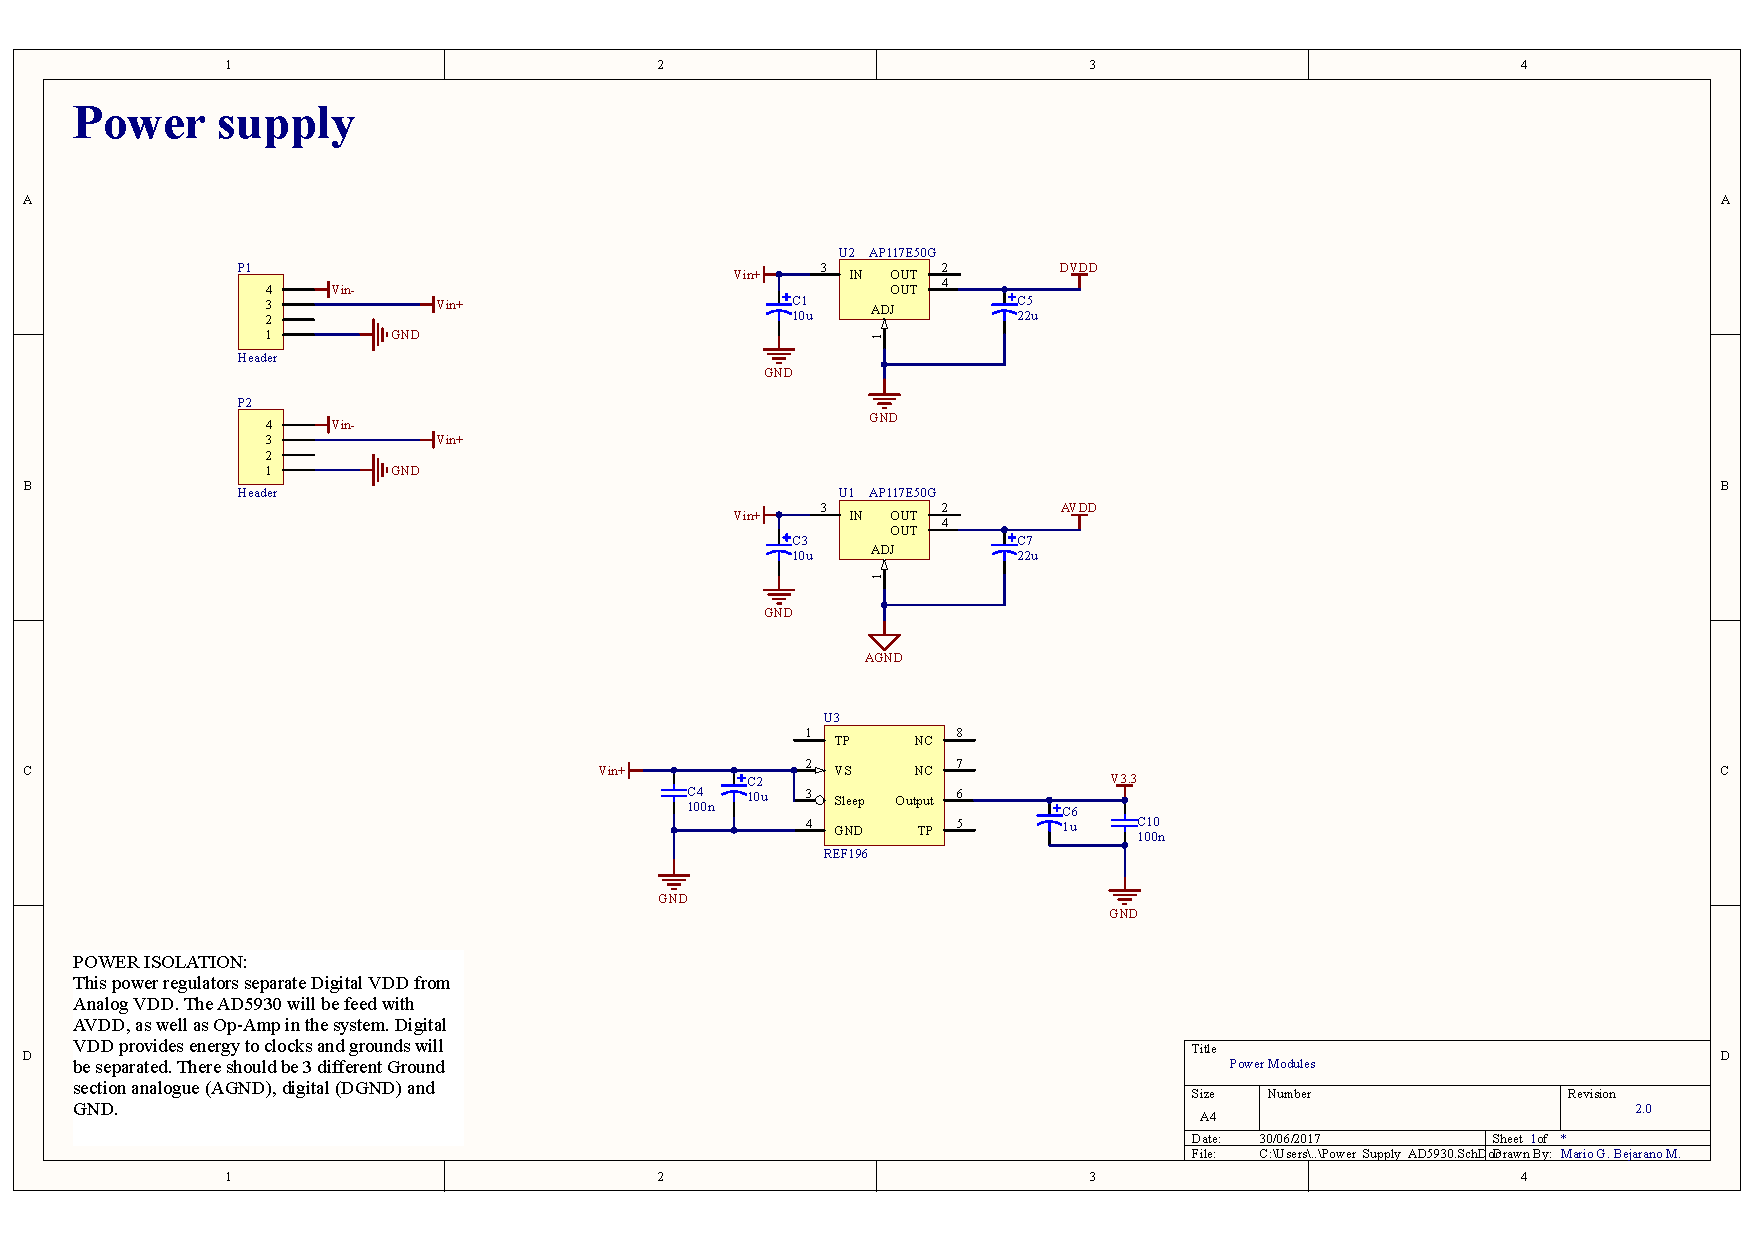
\includegraphics[width=0.9\paperwidth,keepaspectratio,angle=90]{DDS_power_supply}
	\caption[Schematic of the Power supply of the DDS]{The power supply circuit provides 3 different voltages \SI{5}{\volt} for analogue and digital circuitry, and \SI{3}{\volt} for voltage reference. There are three different ground paths for each source. }
	\label{fig:DDS PS}
\end{figure}


\begin{landscape}
	\begin{figure}[!htpb]
		\centering
		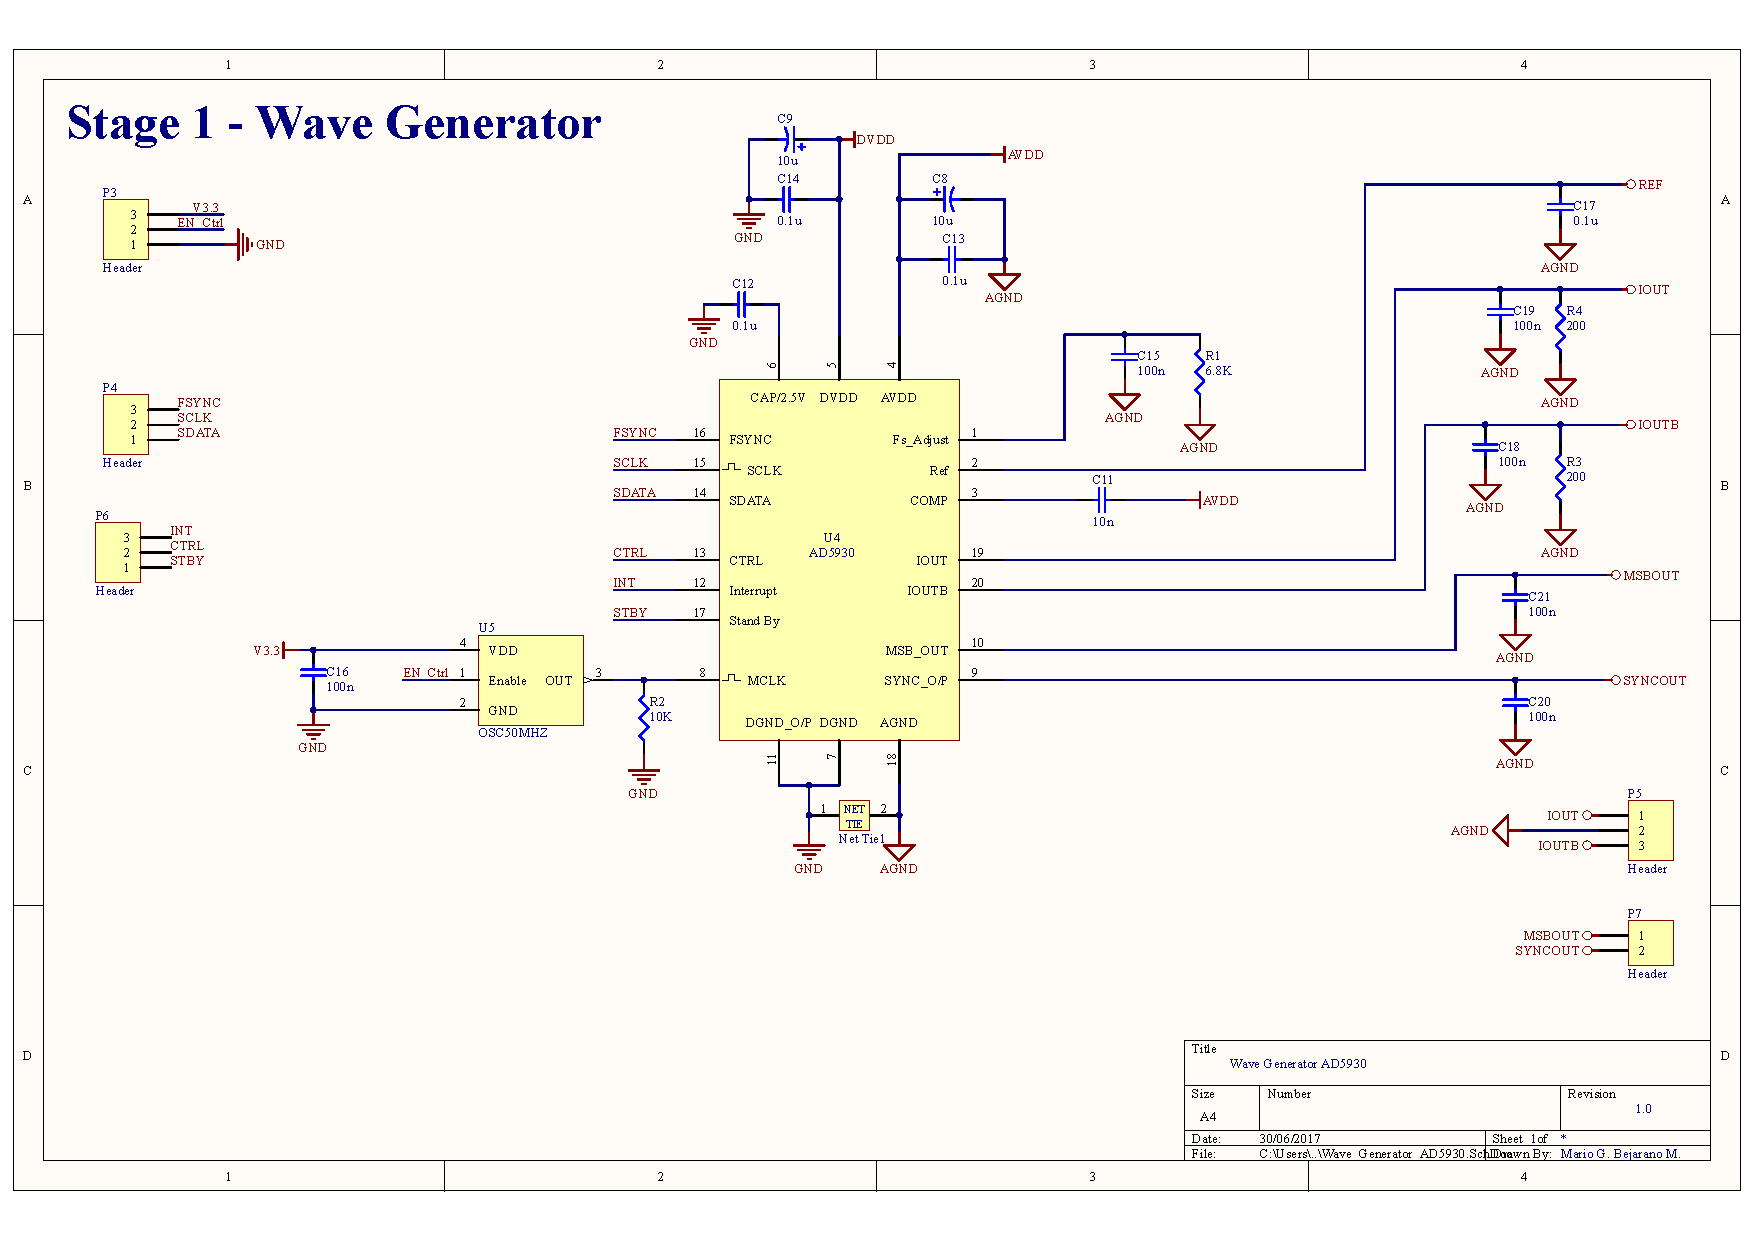
\includegraphics[width=0.9\paperwidth,keepaspectratio]{DDS}
		\caption[Direct digital synthesis circuit schematic]{Schematic of the AD5930, it includes the \SI{50}{\mega\hertz} oscillator and output filters.}
		\label{fig:DDS}
	\end{figure}
\end{landscape}

\section*{Differential gain amplifier}
\label{Appendix: DGA}
\begin{figure}[!htpb]
	\centering
	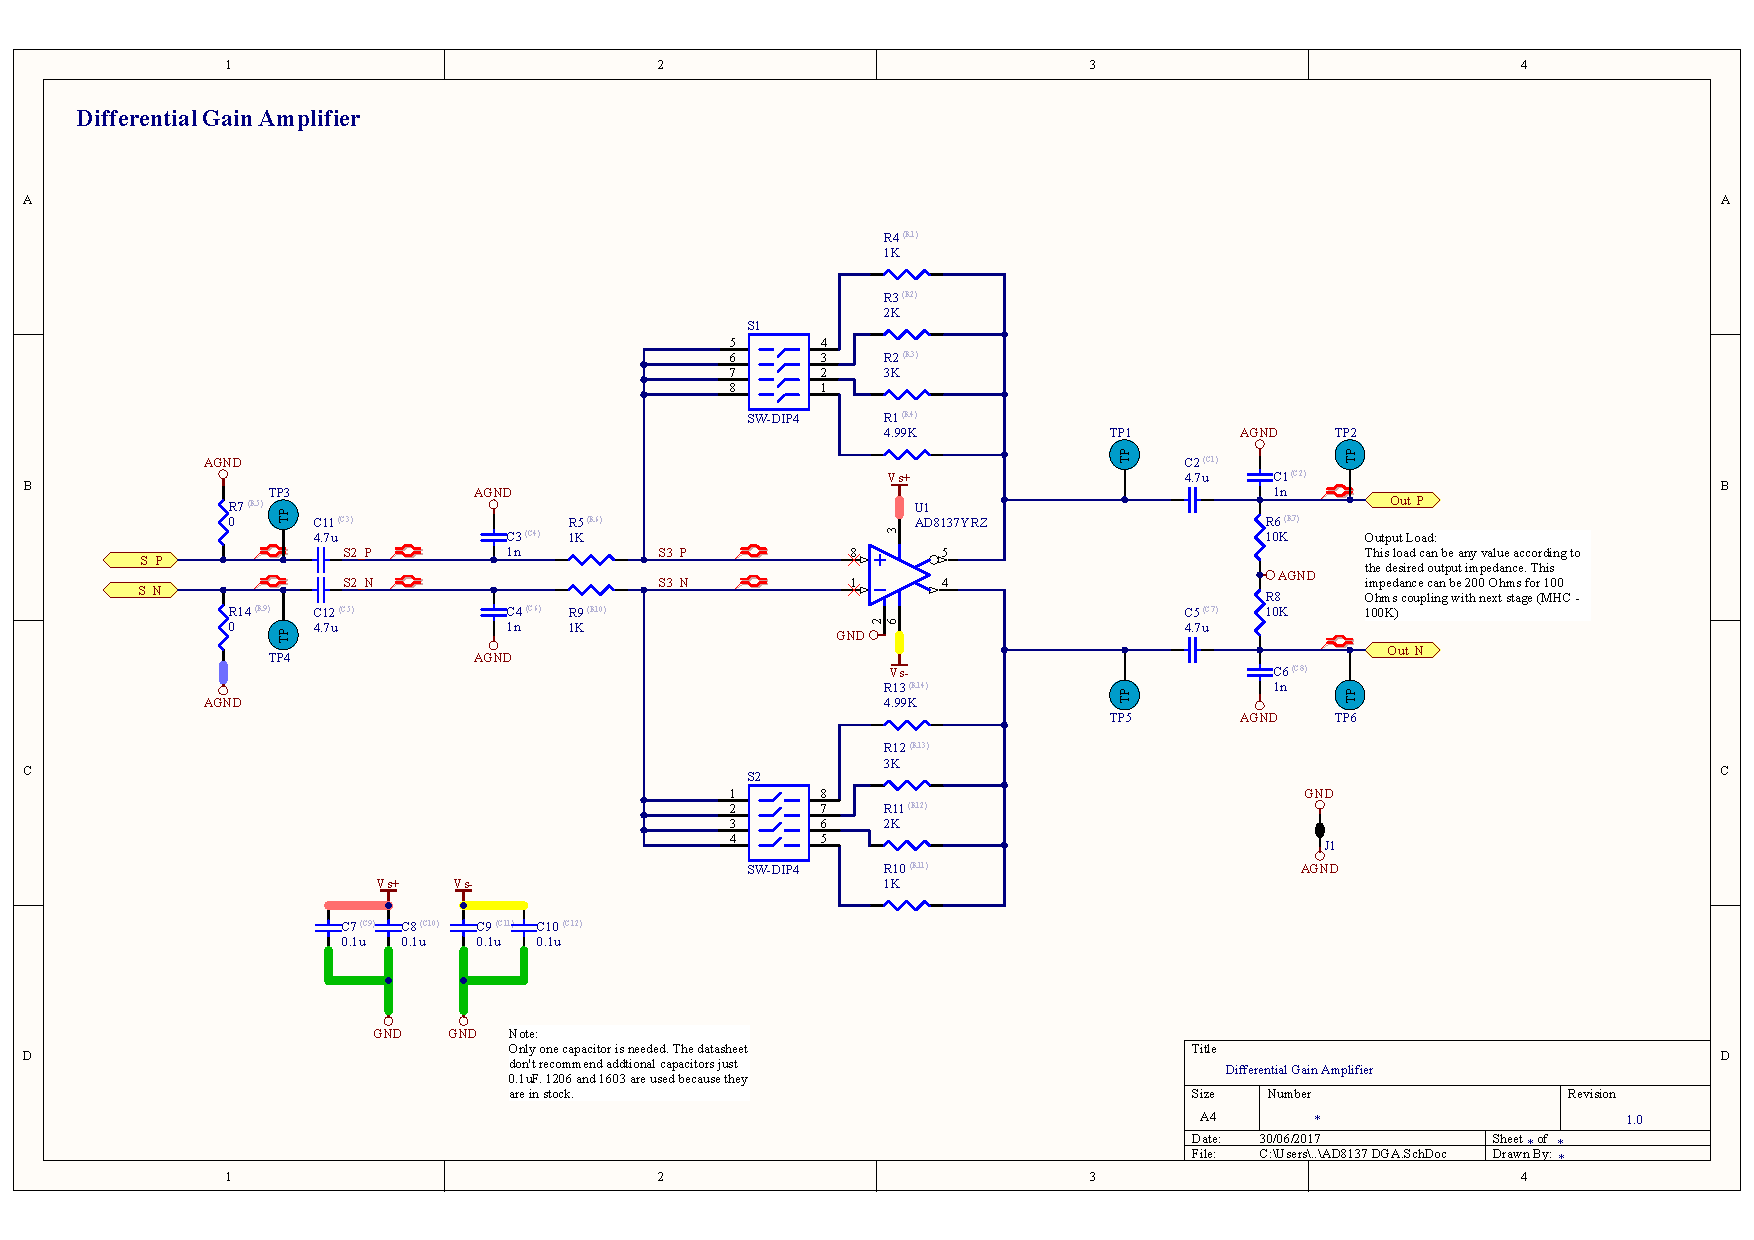
\includegraphics[width=0.9\paperwidth,keepaspectratio,angle=90]{DGA}
	\caption[Schematic of the differential gain amplifier circuit]{Differential gain amplifier controlled by 4 position dip-switch adjusting the gain of the signal output.}
	\label{fig:DGA}
\end{figure}

\begin{landscape}
	\begin{figure}[!htpb]
		\centering
		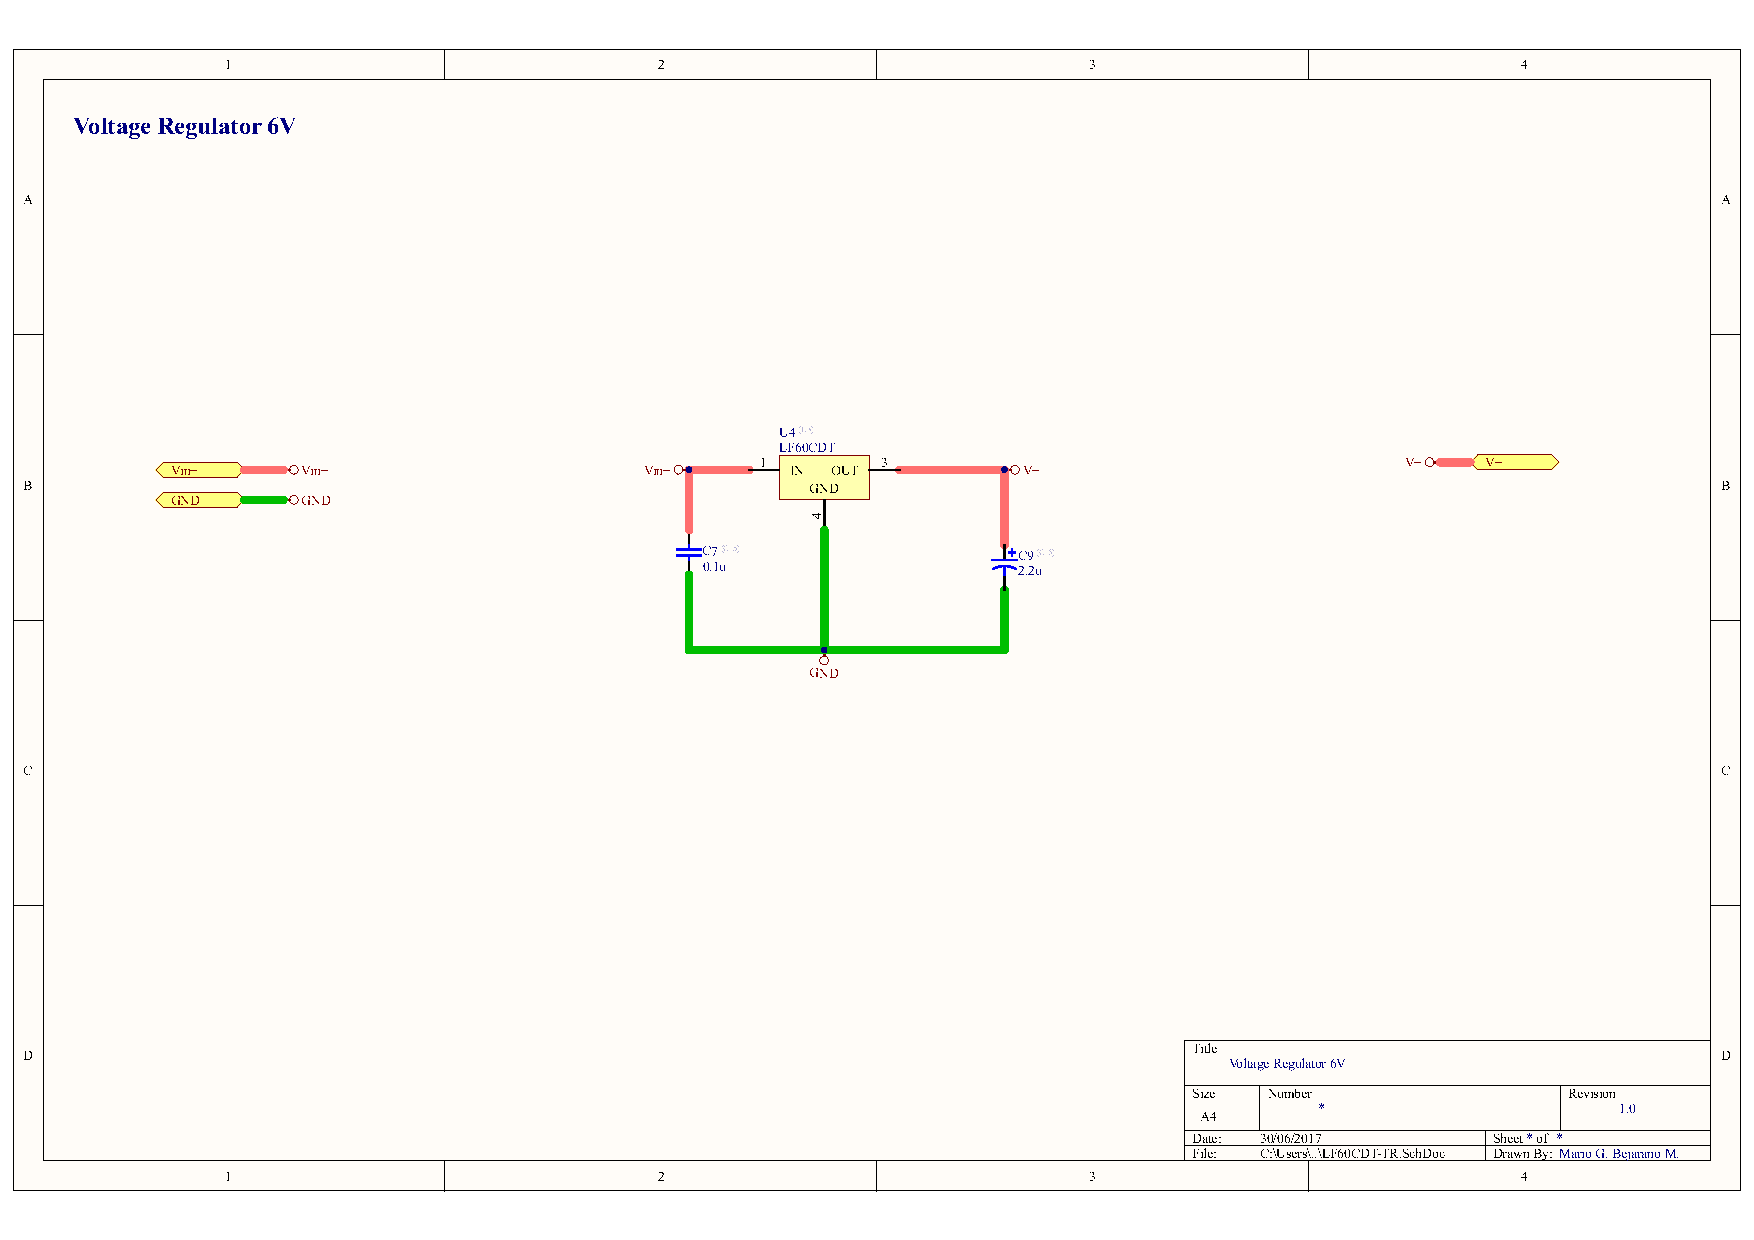
\includegraphics[width=0.9\paperwidth,keepaspectratio]{DGA_PS_6}
		\caption[Positive power supply (\SI{6}{\volt}) for the differential amplifier]{Power supply circuit based on the IC LF60CDT.}
		\label{fig:DGA PS 6}
	\end{figure}
\end{landscape}

\begin{landscape}
	\begin{figure}[!htpb]
		\centering
		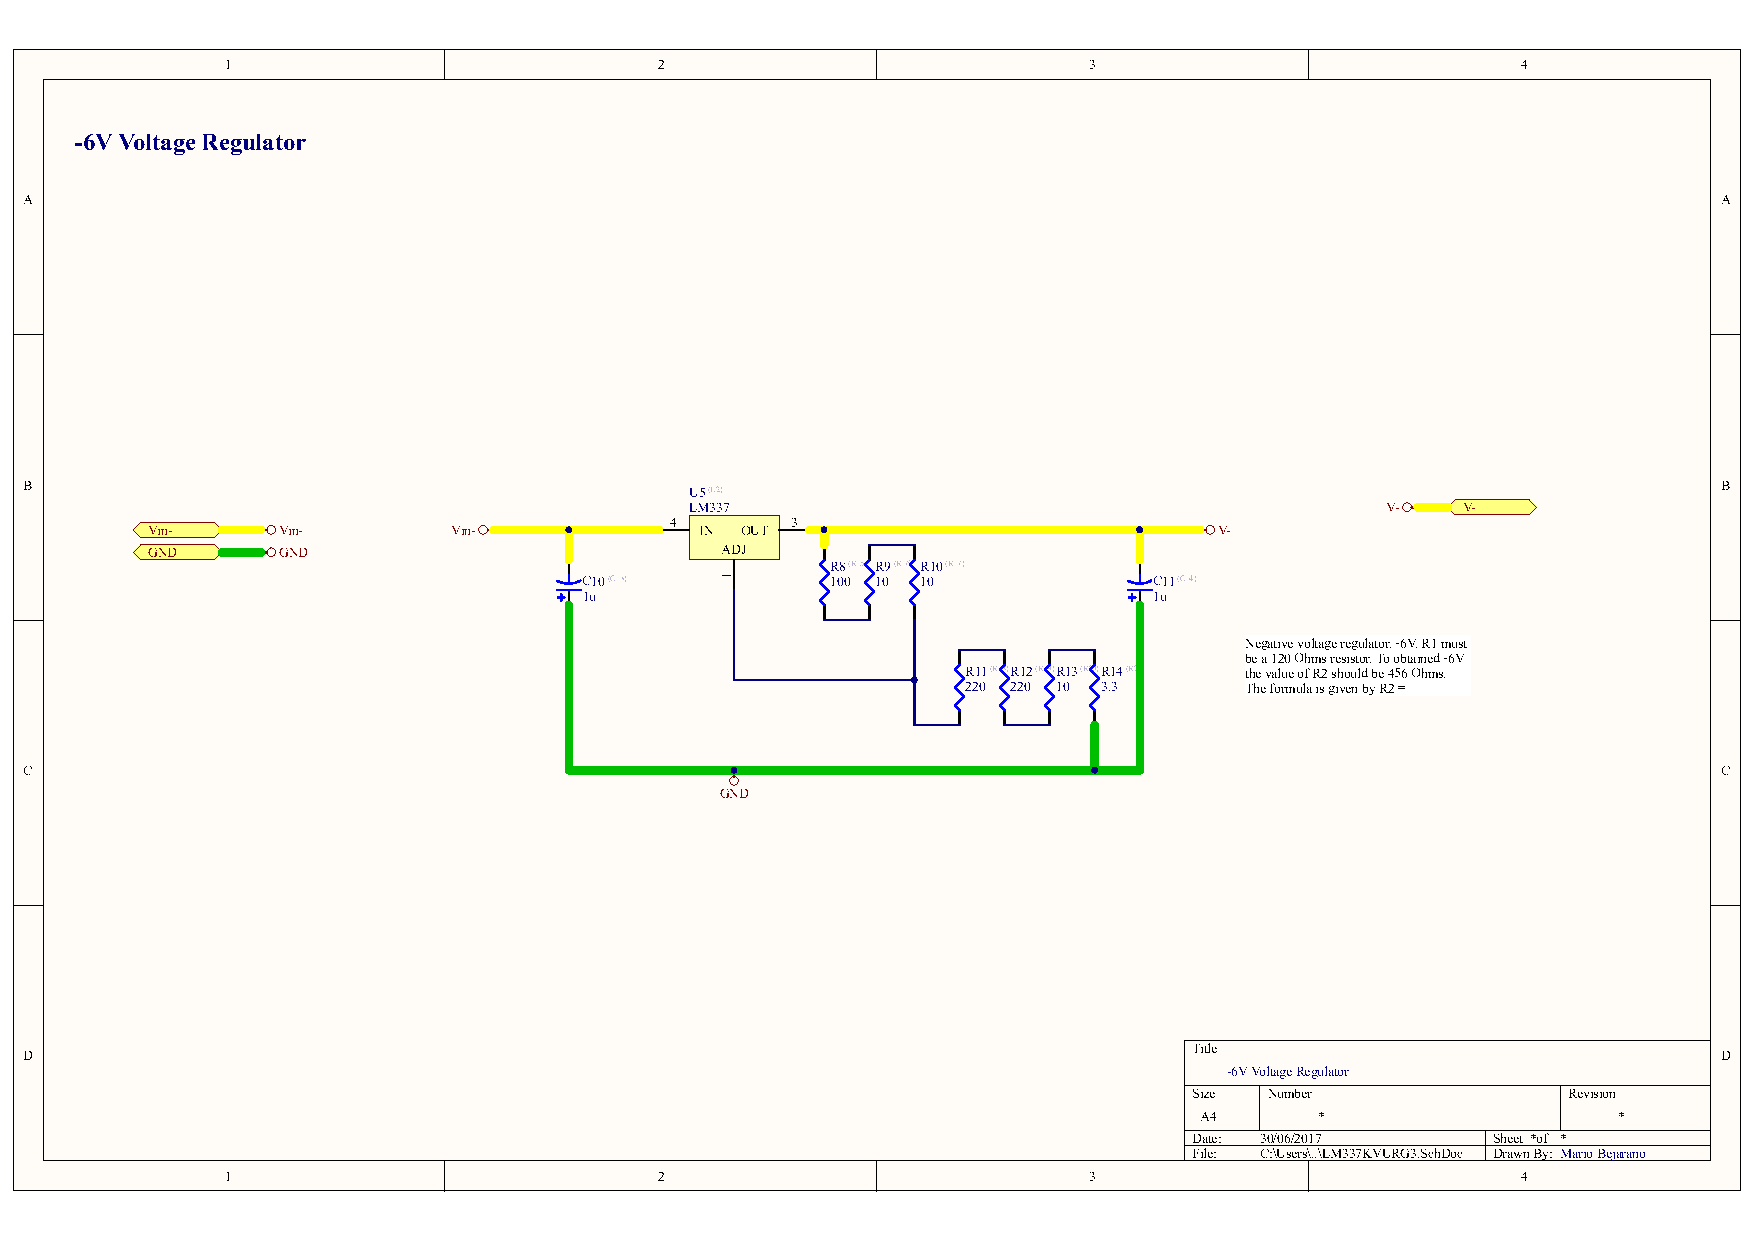
\includegraphics[width=0.9\paperwidth,keepaspectratio]{DGA_PS_N6}
		\caption[Negative power supply (\SI{-6}{\volt}) for the differential amplifier]{Power supply circuit based on the IC LM337, the resistors were adjusted to achieve -\SI{6}{\volt}.}
		\label{fig:DGA PS -6}
	\end{figure}
\end{landscape}

\section*{Modified Howland circuit}
\label{Appendix: MHC}
\begin{figure}[!htpb]
	\centering
	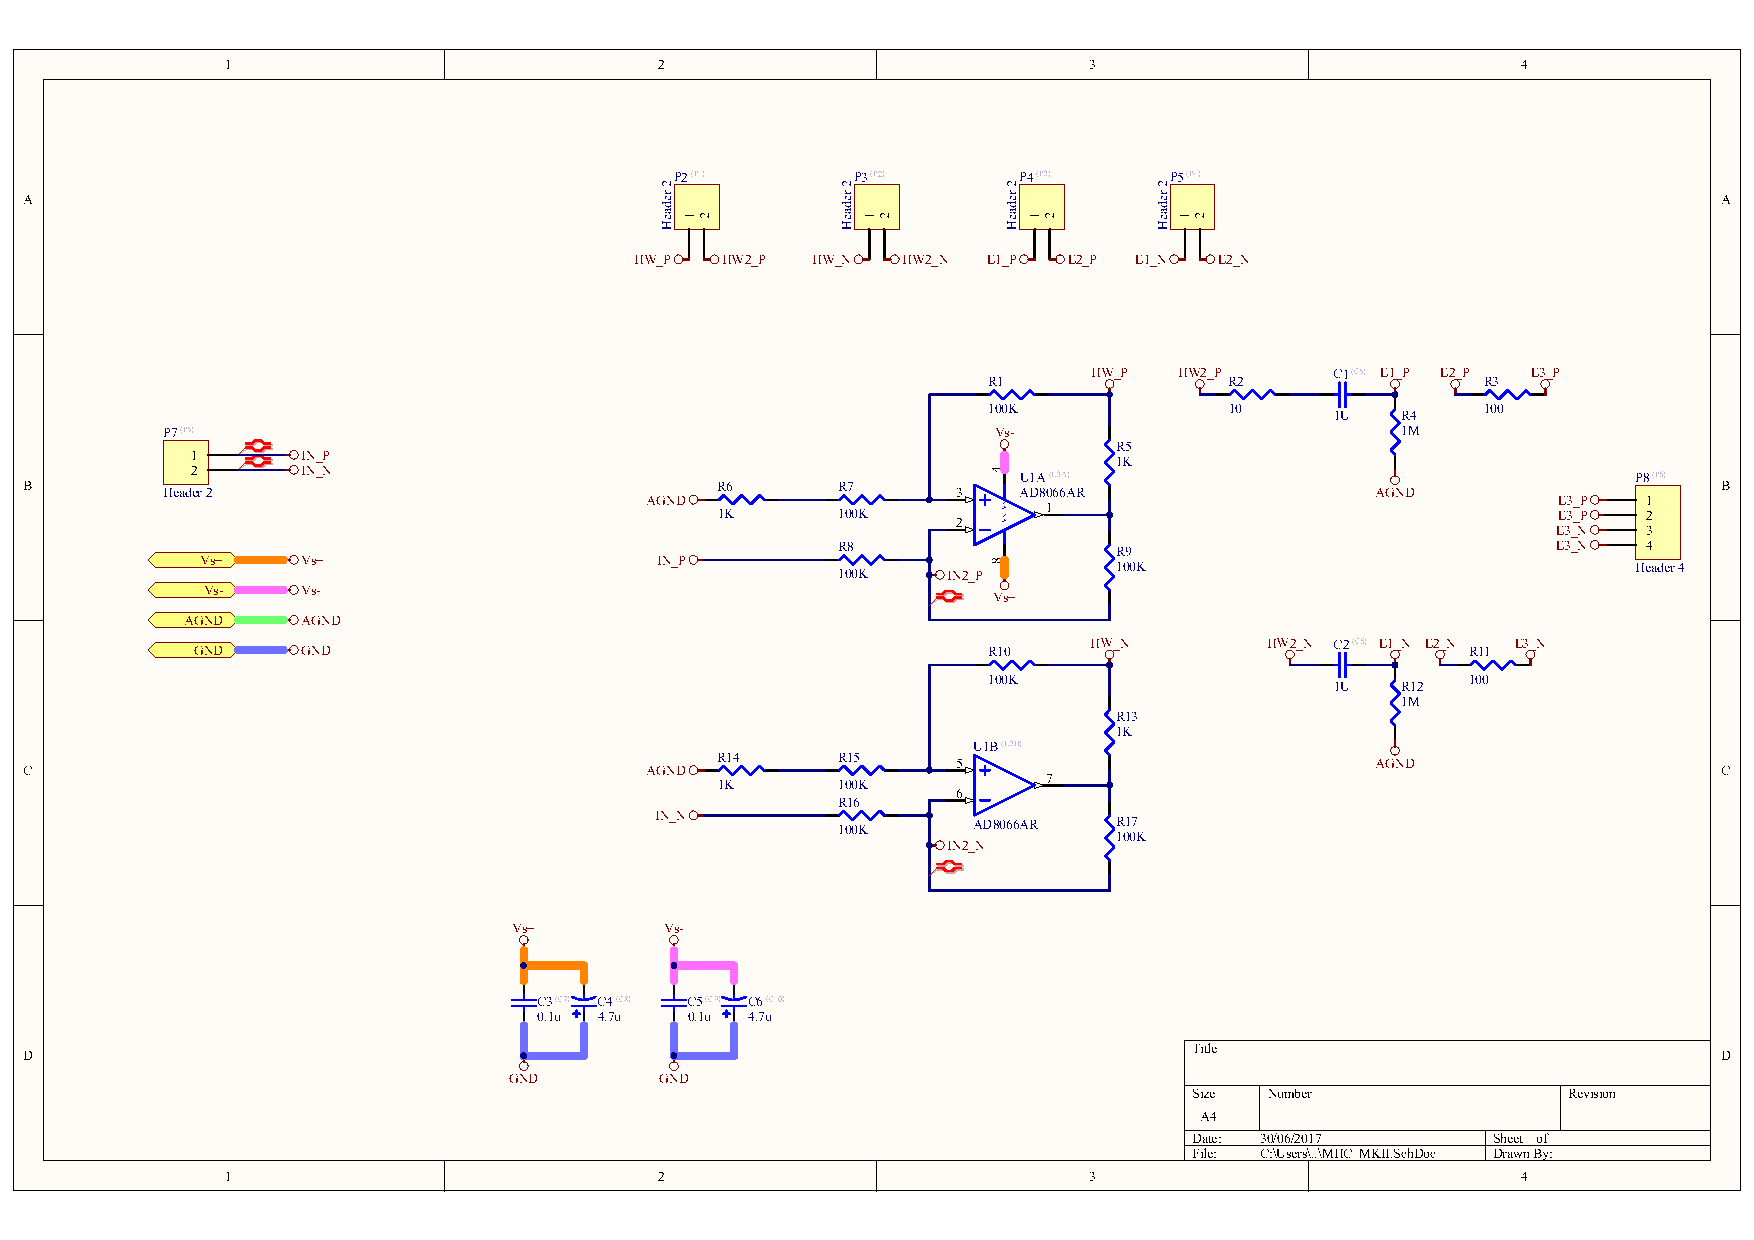
\includegraphics[width=0.9\paperwidth,keepaspectratio,angle=90]{MHC}
	\caption[Schematic of the differential gain amplifier circuit]{Differential gain amplifier controlled by 4 position dip-switch adjusting the gain of the signal output.}
	\label{fig:MHC}
\end{figure}

\begin{landscape}
	\begin{figure}[!htpb]
		\centering
		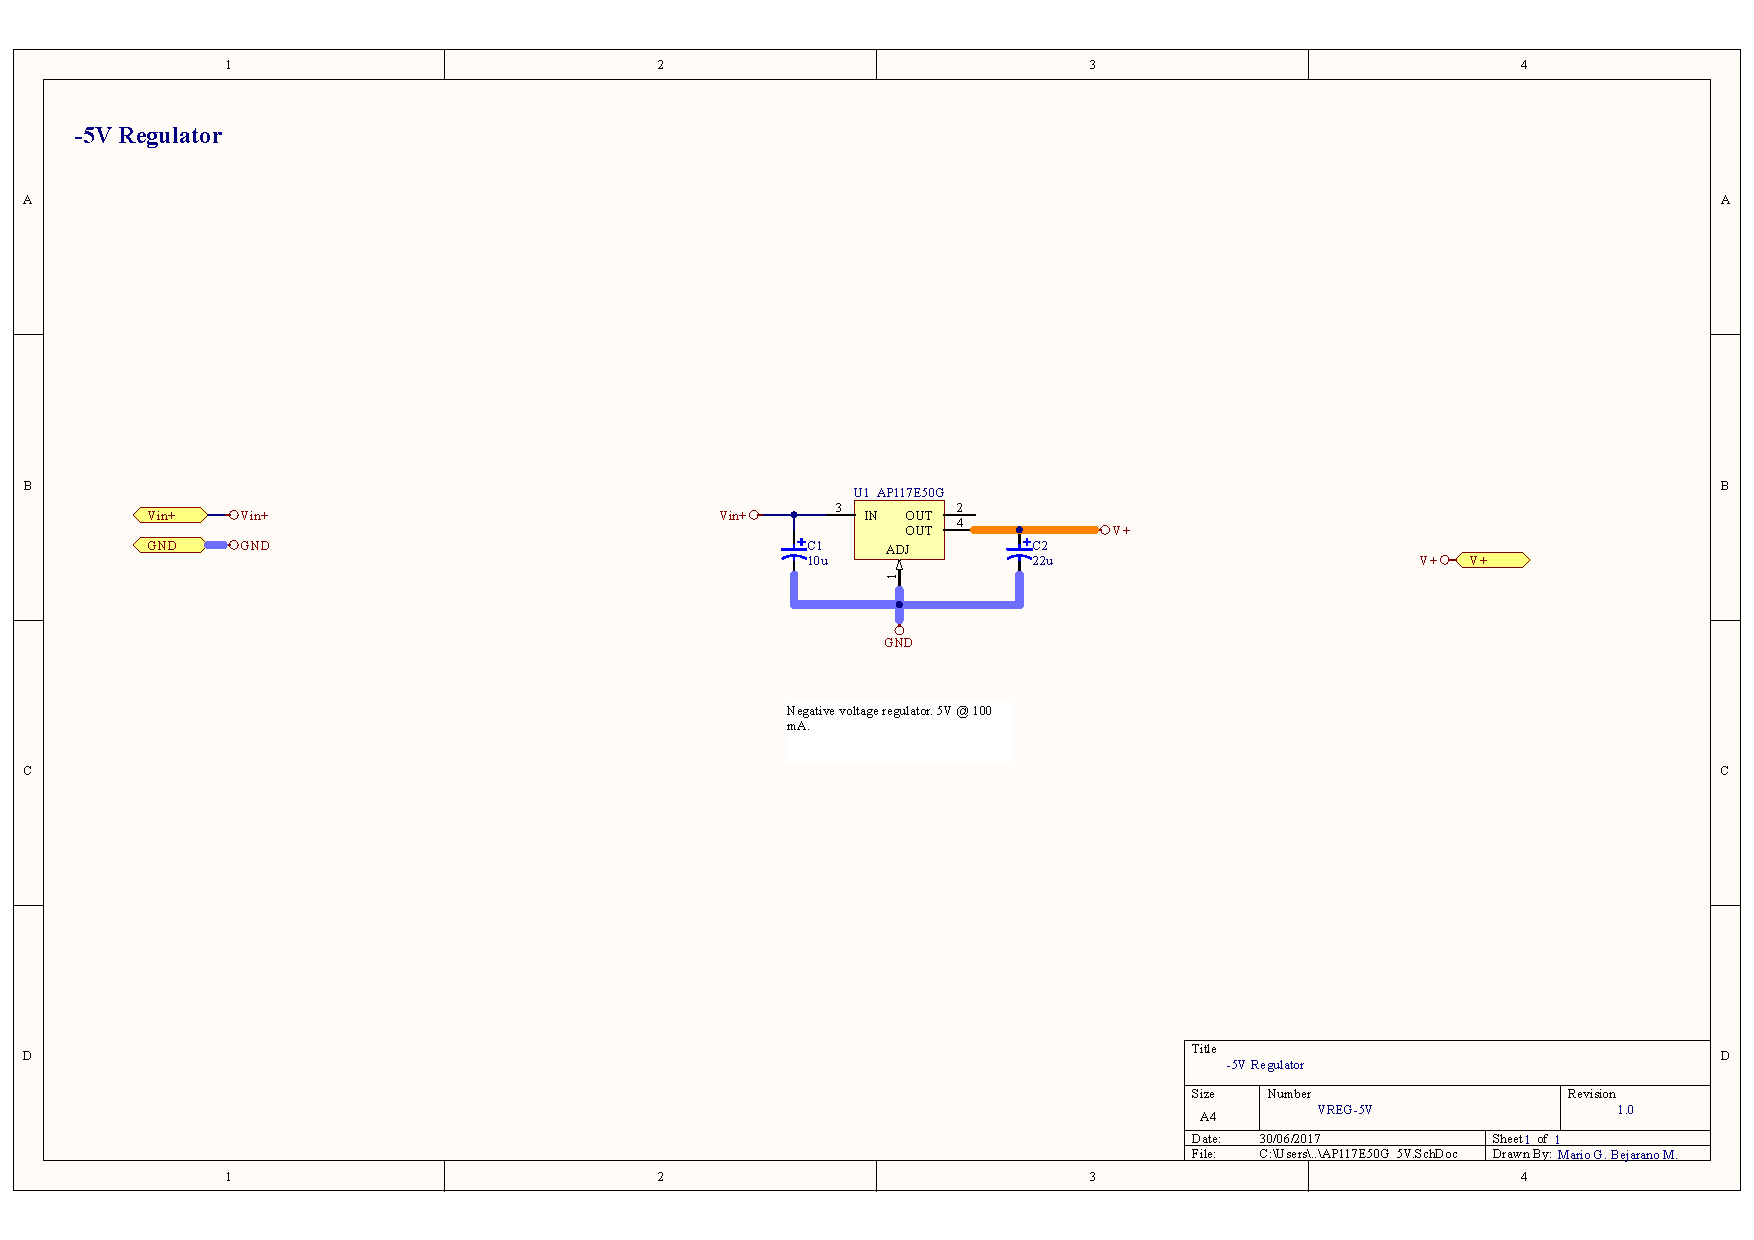
\includegraphics[width=0.9\paperwidth,keepaspectratio]{MHC_PS_5}
		\caption[Positive power supply (\SI{5}{\volt}) for the modified Howland circuit]{Power supply circuit based on the IC AP117E50G.}
		\label{fig:MHC PS 5}
	\end{figure}
\end{landscape}

\begin{landscape}
	\begin{figure}[!htpb]
		\centering
		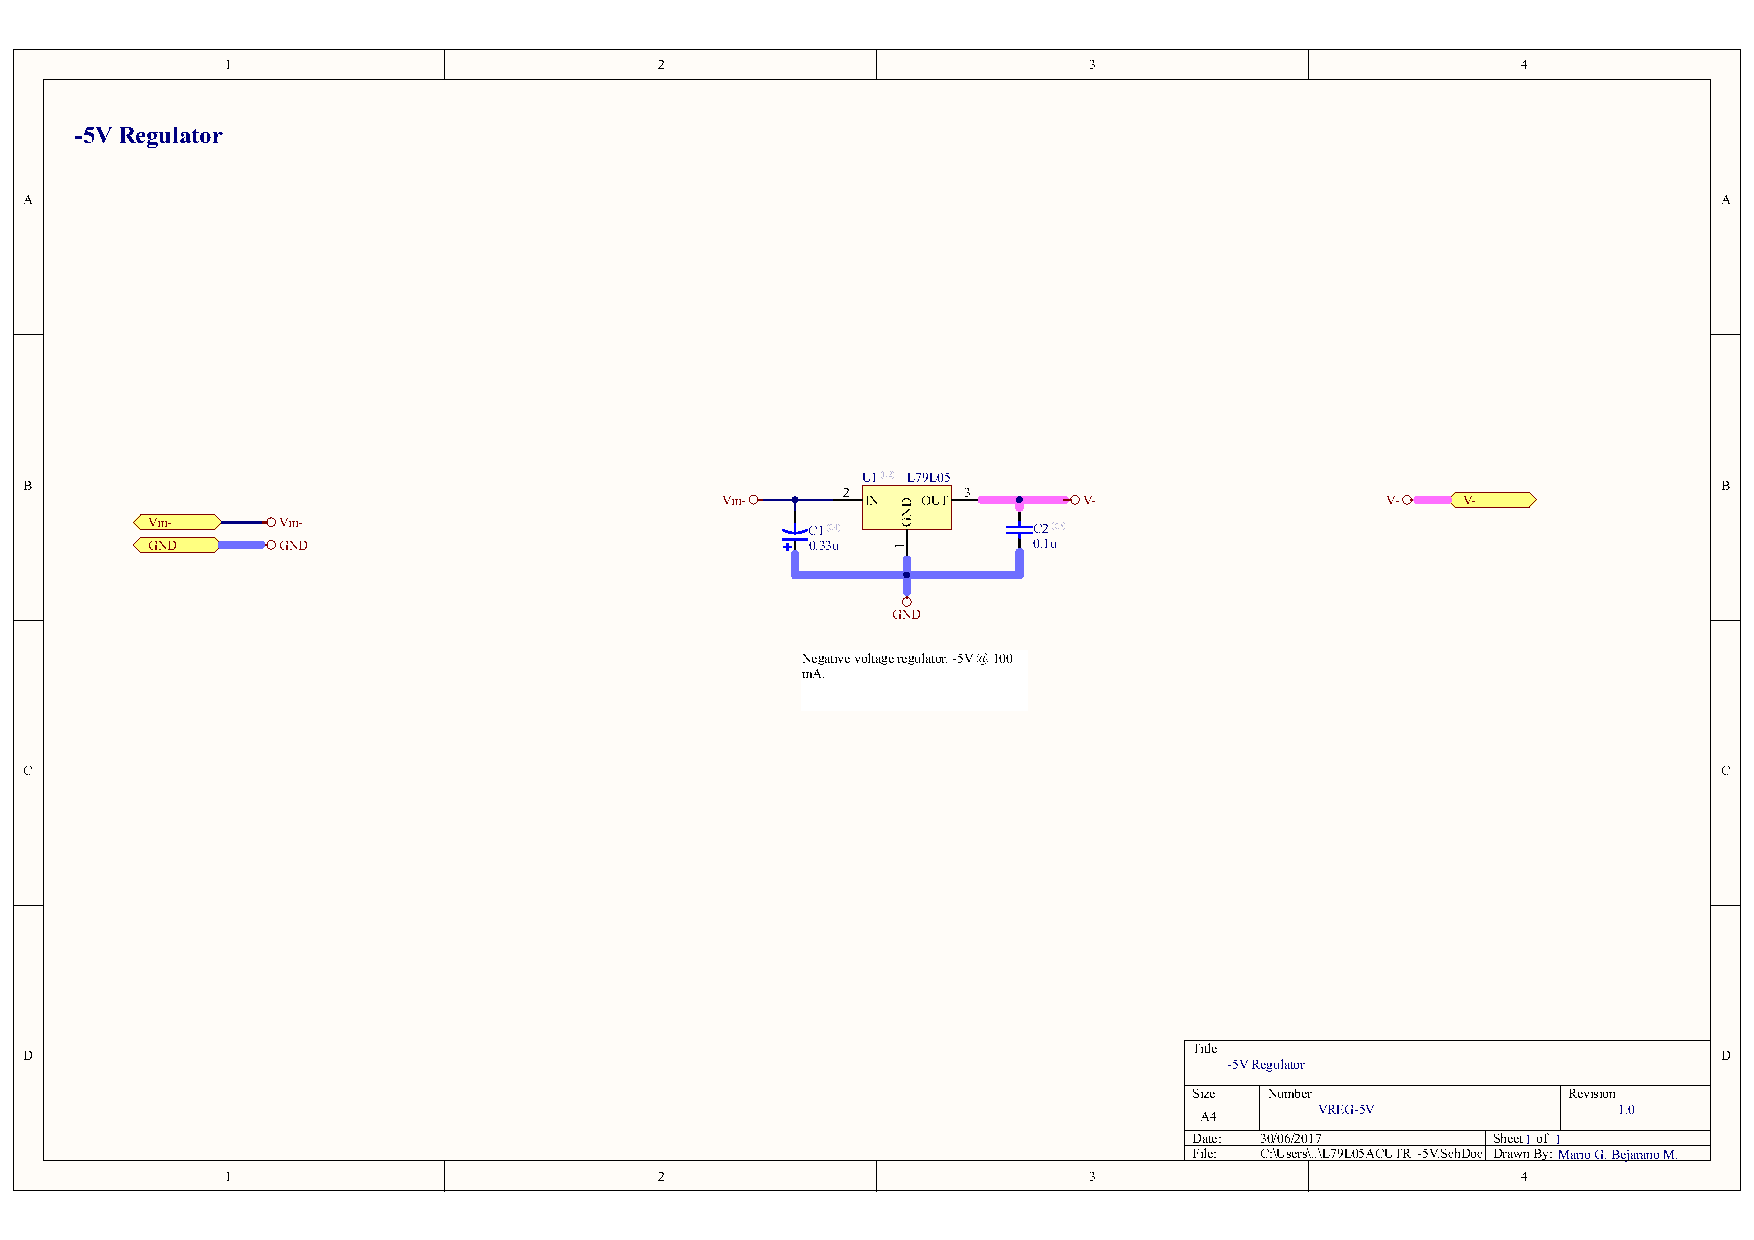
\includegraphics[width=0.9\paperwidth,keepaspectratio]{MHC_PS_N5}
		\caption[Negative power supply (\SI{-5}{\volt}) for the modified Howland circuit]{Power supply circuit based on the fixed voltage regulator (-\SI{5}{\volt}) IC L79L05.}
		\label{fig:MHC PS -5}
	\end{figure}
\end{landscape}

\section*{Voltage sense circuit}
\label{Appendix: VSense}
\begin{figure}[!htpb]
	\centering
	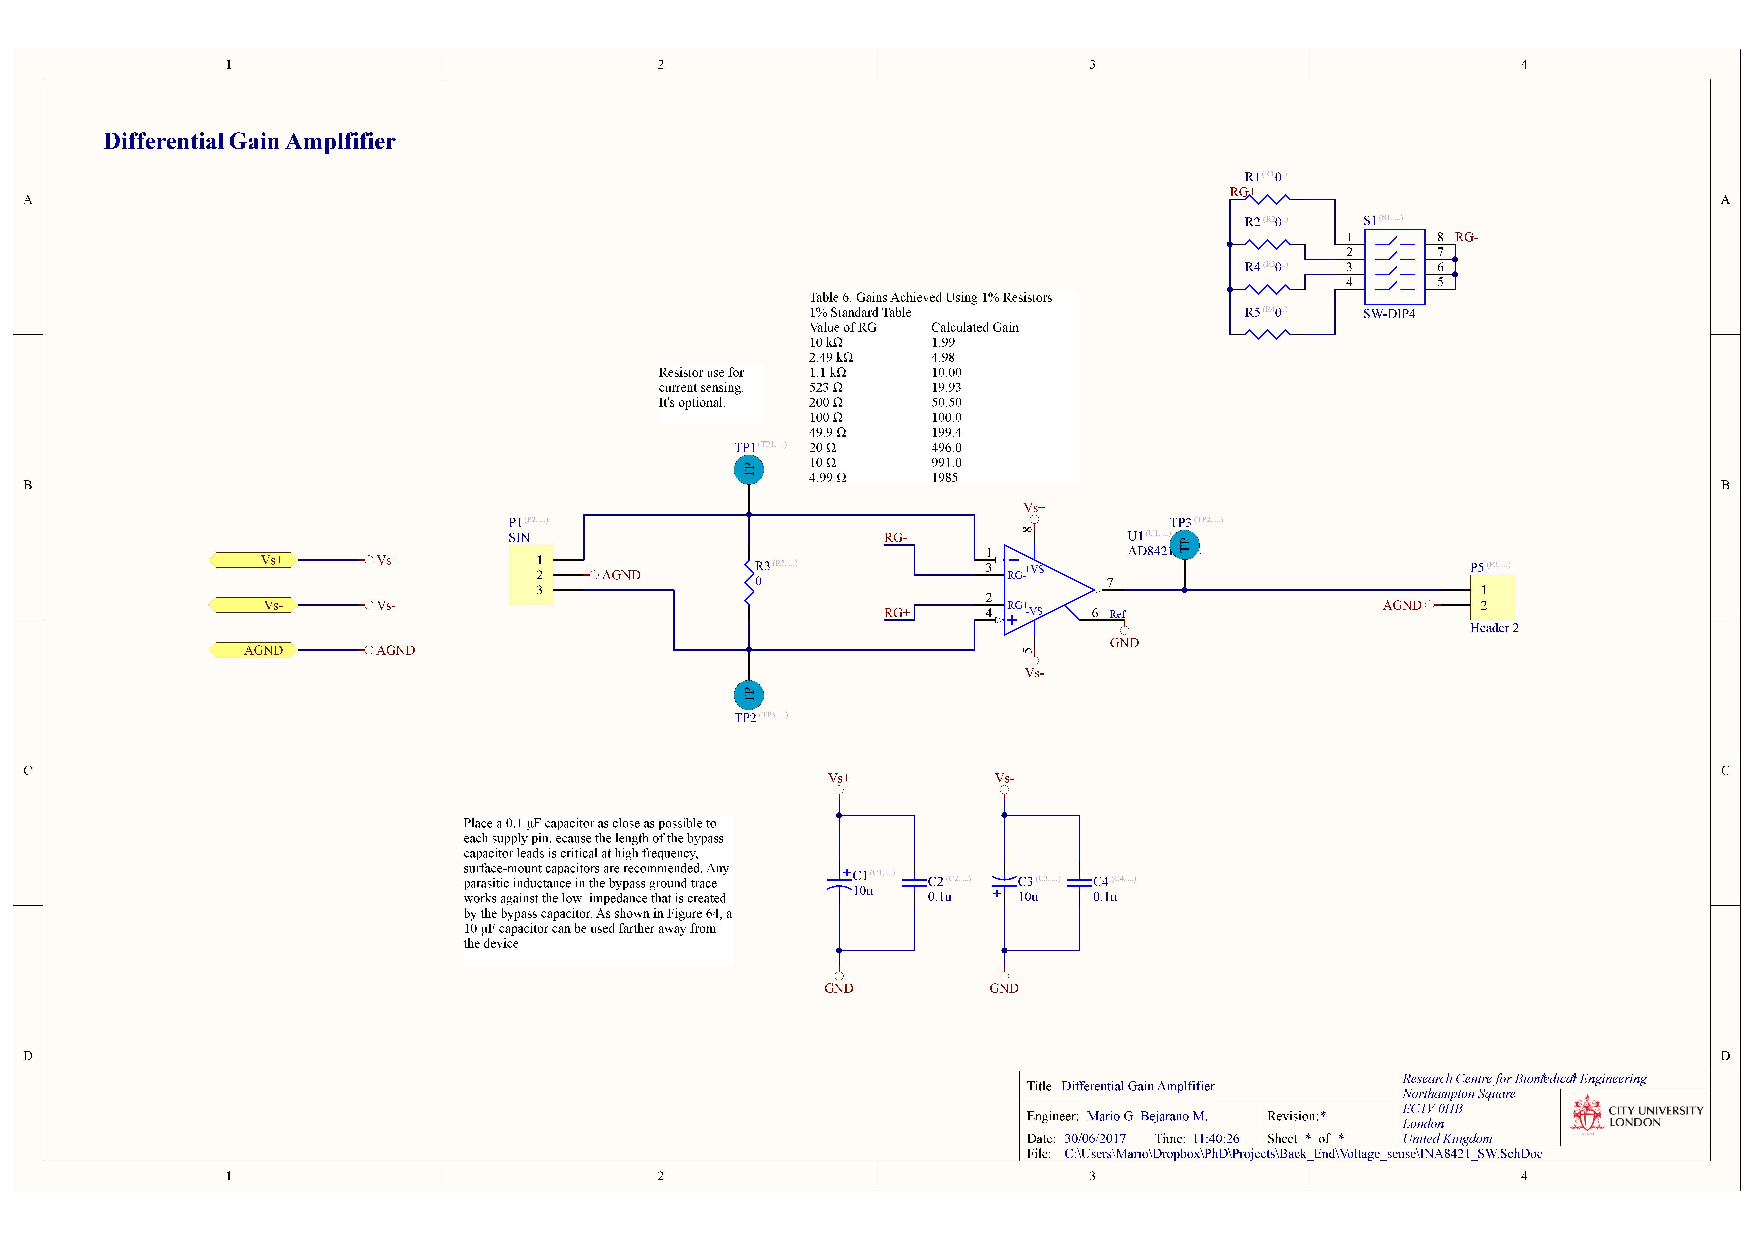
\includegraphics[width=0.9\paperwidth,keepaspectratio,angle=90]{VSense}
	\caption[Schematic of the voltage sense circuit]{The voltage sense circuit sense voltage from an unknown source. This same circuit was used to sense the current driven by the MHC, as well as the potential from the load under test (unknown $Z$).}
	\label{fig:Voltage sense}
\end{figure}

\section*{Envelope detection circuits}
\label{Appendix: Envelope}
\begin{figure}[!htpb]
	\centering
	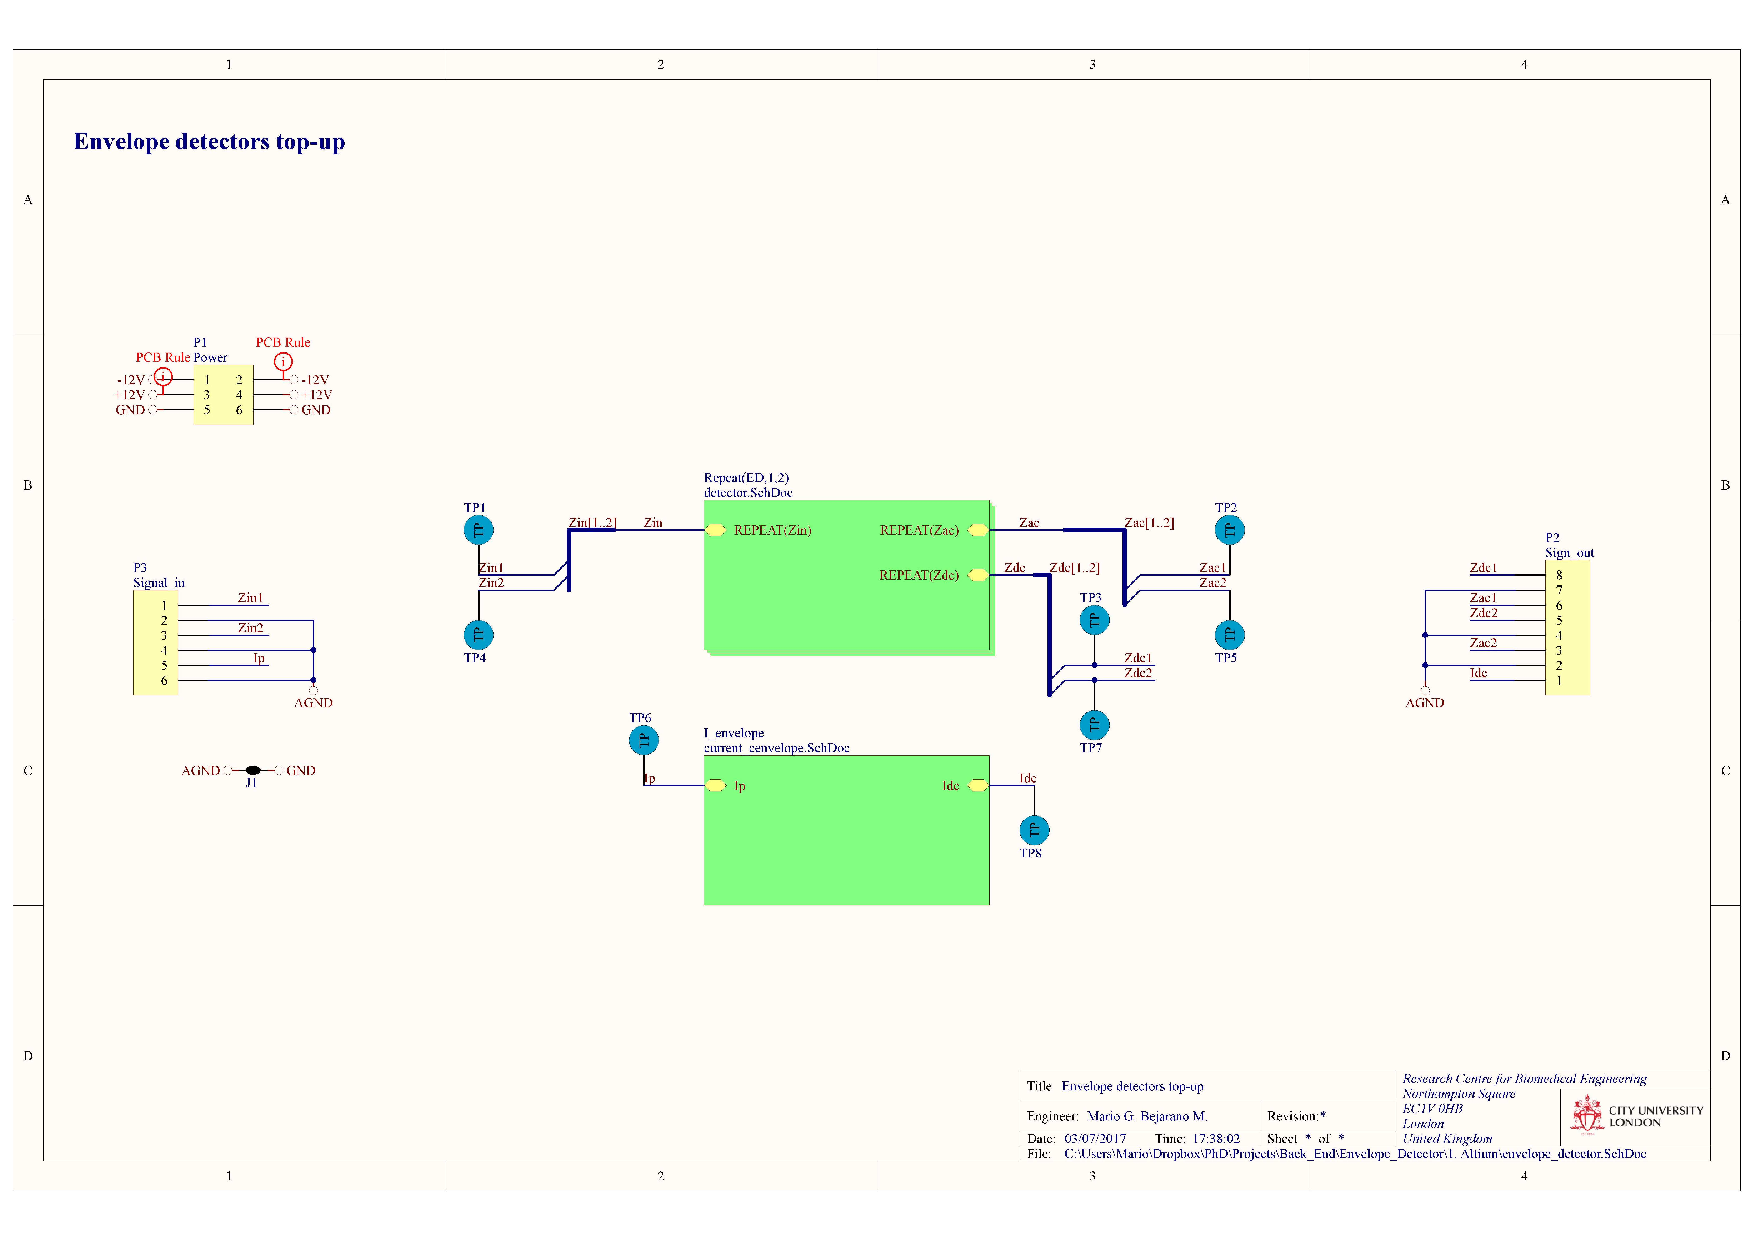
\includegraphics[width=0.9\paperwidth,keepaspectratio,angle=90]{env_det_top}
	\caption[Top-up schematic of the envelope detector circuits]{The iPG device has designed to work with two voltage channels ans one current channels sensor. Each envelope detector extracts the peak detection, which output is passed to the output ports of the device.}
	\label{fig:envelope detector top}
\end{figure}

\begin{landscape}
	\begin{figure}[!htpb]
		\centering
		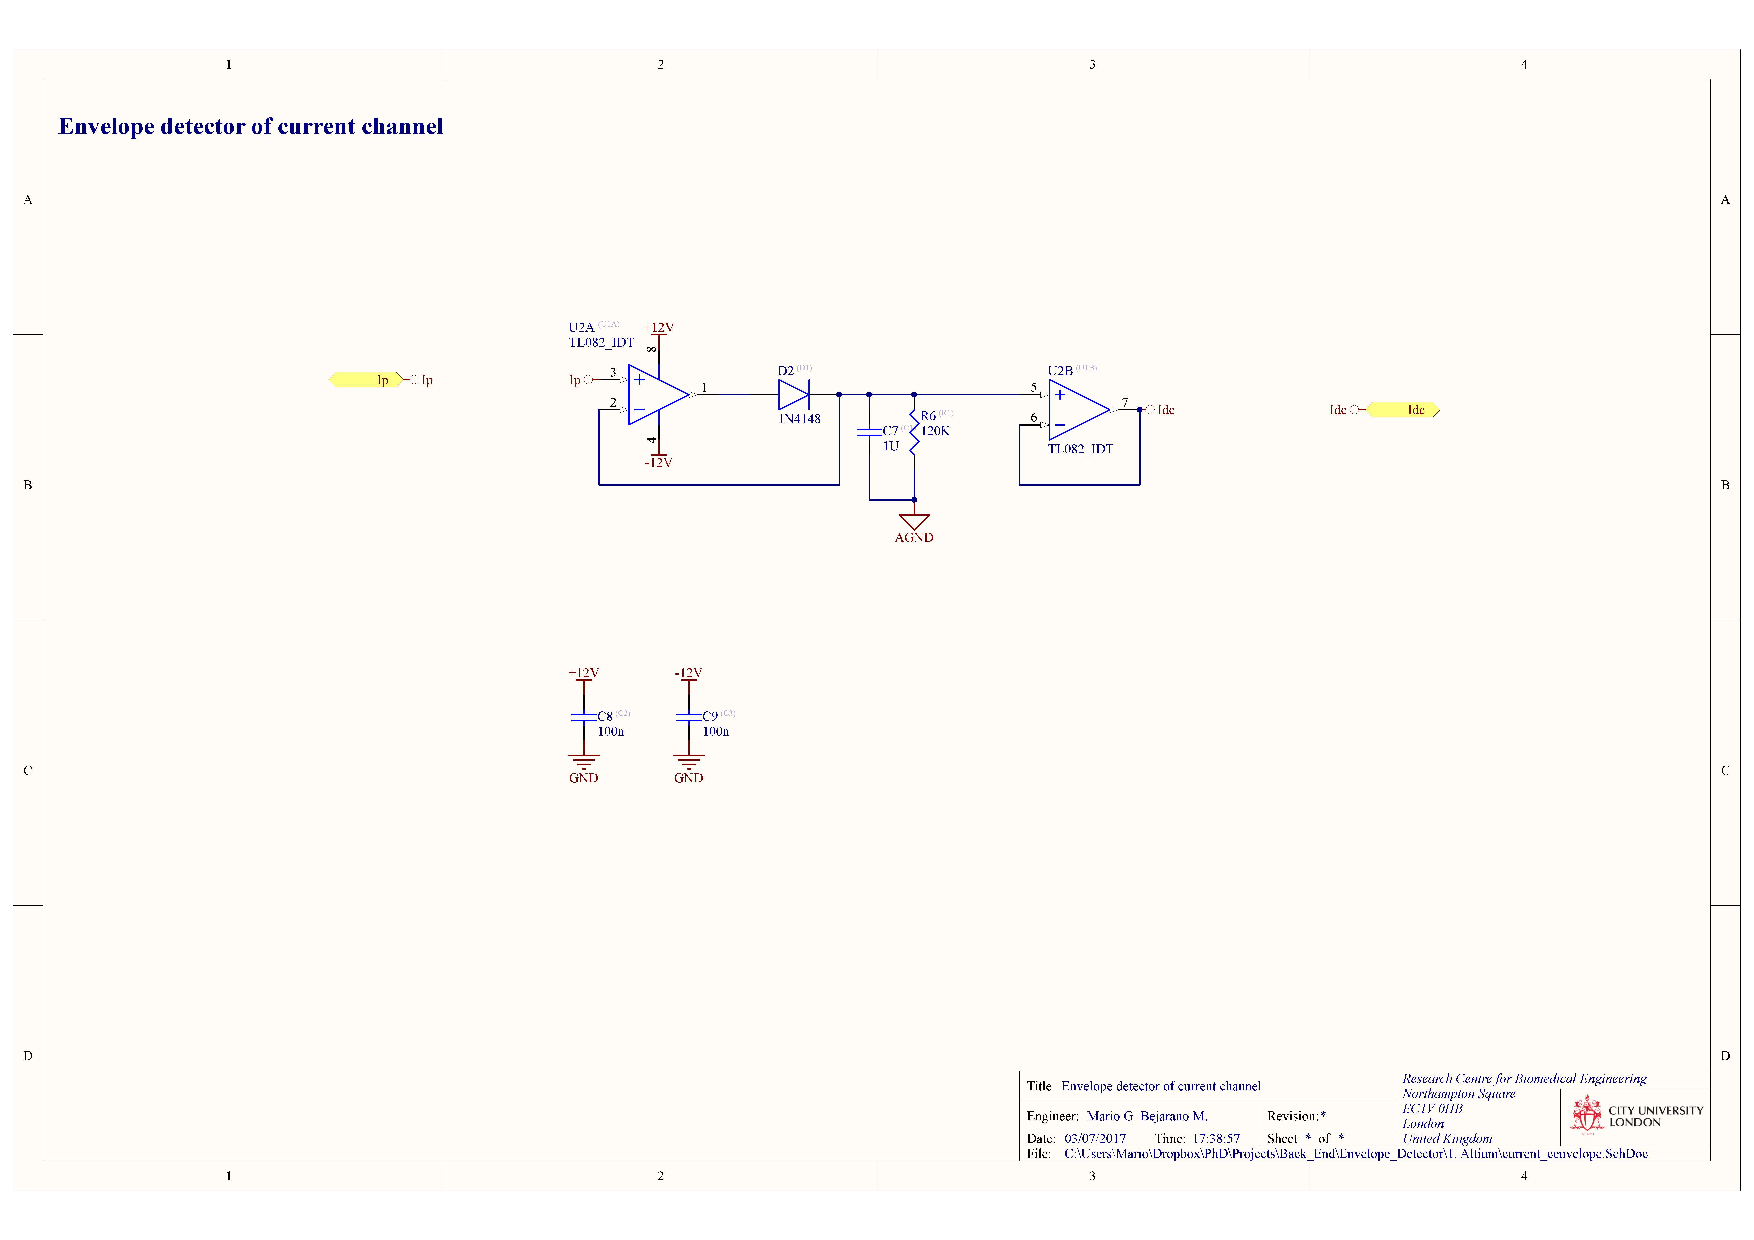
\includegraphics[width=0.9\paperwidth,keepaspectratio]{env_det_curr}
		\caption[Envelope detector of the current channel]{The current of the MHC is converted to voltage which later can be detected by this circuit. The voltage detected from the current drives consist of a perfect diode configuration based on a TL084 and a diode 1N4148. Then the signal is sampled and hold by a capacitor.The output is buffered to get a low impedance output.}
		\label{fig:envelope detector current}
	\end{figure}
\end{landscape}

\begin{landscape}
	\begin{figure}[!htpb]
		\centering
		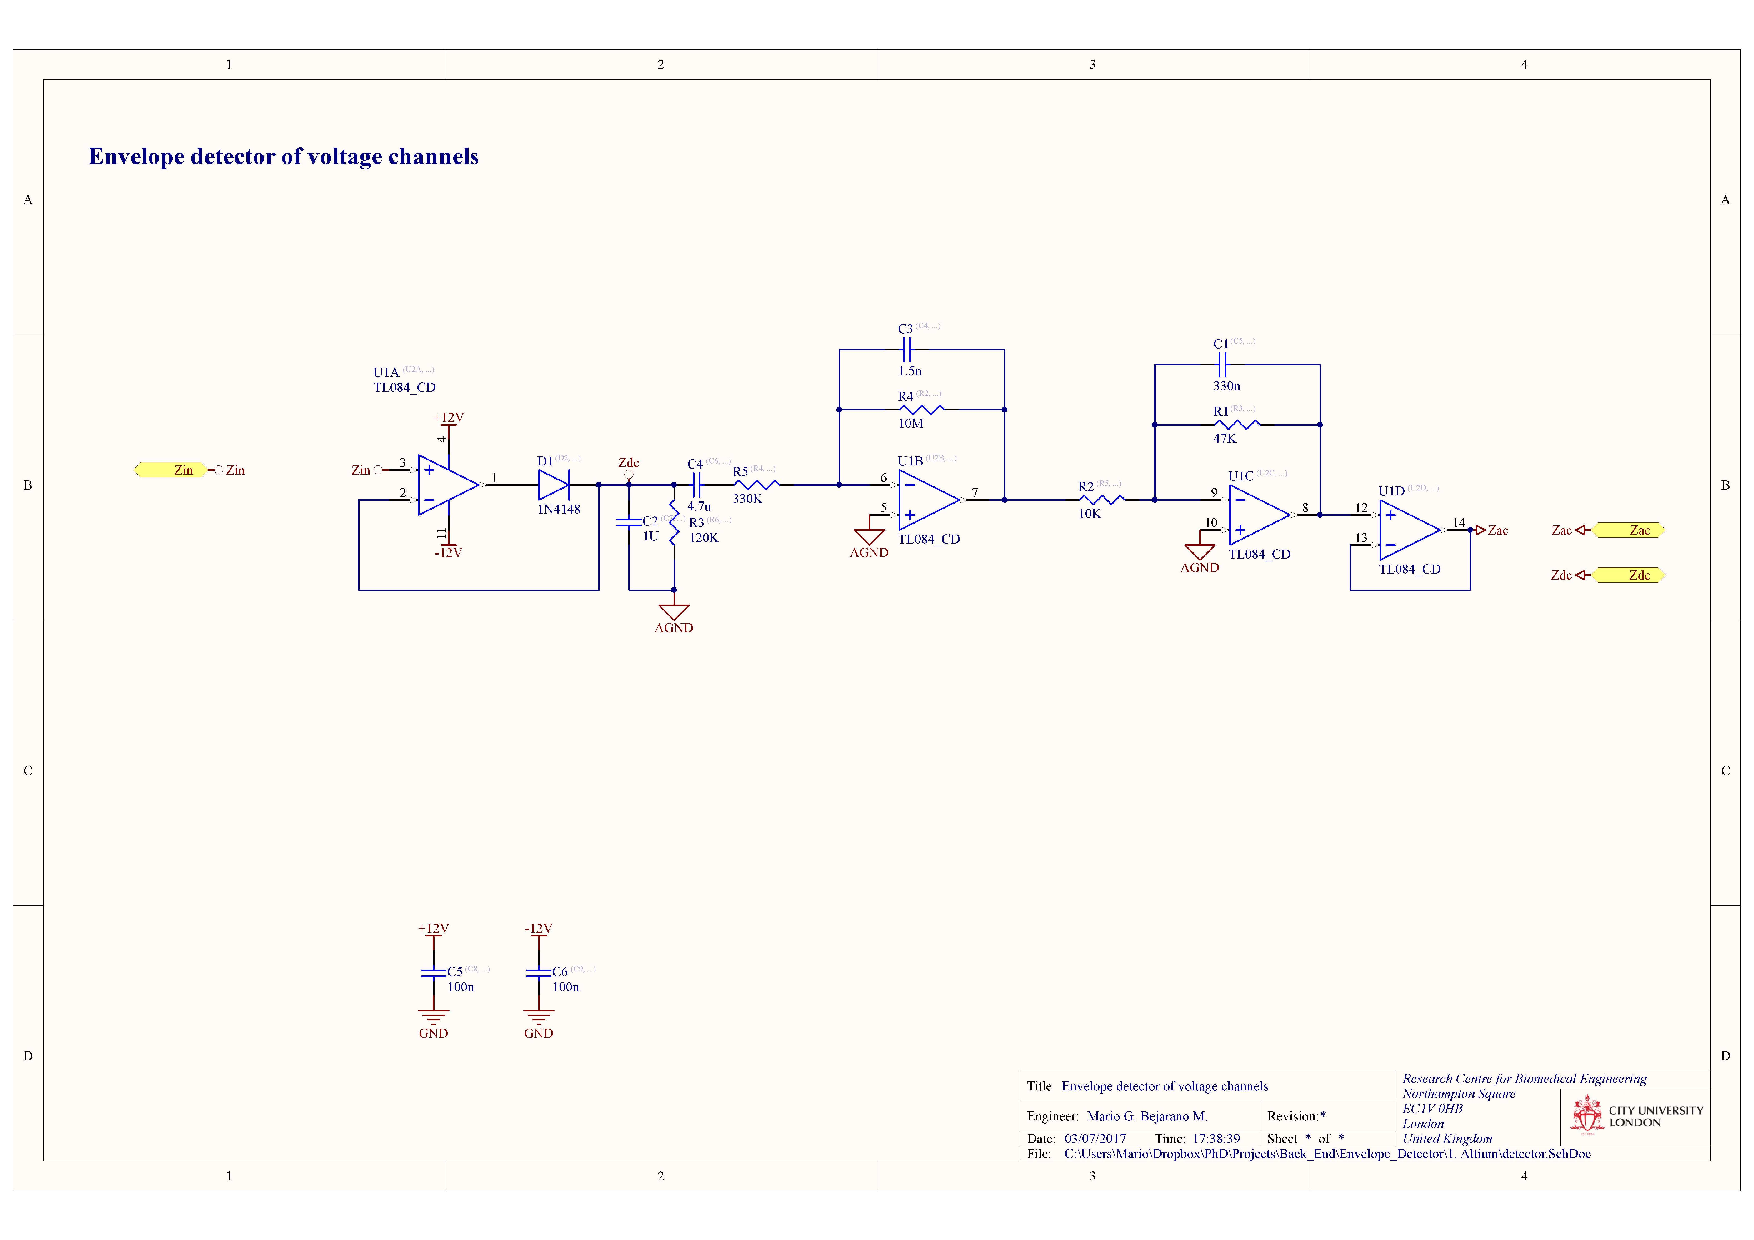
\includegraphics[width=0.95\paperwidth,keepaspectratio]{env_det_volt}
		\caption[Envelope detector of the voltage channels]{The voltage detector consist of a perfect diode configuration based on a TL084 and a diode 1N4148. Then the signal is sampled and hold by a capacitor. The output of this signal is later passed to a band-pass filter and a buffer.}
		\label{fig:envelope detector voltage}
	\end{figure}
\end{landscape}
